\chapter{Constructing landscape-level risk-maps}

Previously in Chapter \ref{ch5:dispersal-model}, we considered a generic $SIR$ dispersal model that spread with non-local dispersal. 
Constructing a non-local dispersal model resolved the major problem witnessed in Chapter \ref{fig:ch4_uk_spread}, namely, the failure of the SLM to spread on a realistic host density. 
However, the findings of Chapter \ref{ch5:dispersal-model} lacked biological specificity.
The present chapter aims construct a simplified model of ash dieback, capturing only the essential dynamics of wind-borne dispersal.

A seasonal-based $SEIR$-like model is developed to simulate the natural wind-dispersal mechanism of ash dieback at local-spatial scales. 
A novel framework is then developed to spatially-scale up the small-scale $SEIR$-based epidemic model over Great Britain using a modelled ash canopy cover data-set \cite{hill.data}.
The framework is largely generic, and could in principle be adapted for any dispersal-based tree pathosystem\textemdash provided a sufficient host abundance data-set.
Combining two models at different spatial scales has clear analogies to a sub-grid model \cite{sub-grid}.
 
To measure invasiveness, a spatially-explicit reproductive ratio, denoted by $R_0$, is computed from model simulations.
The wind-dispersal model of ADB brings together key elements presented in chapter \ref{ch5:dispersal-model} i.e. measuring $R_0$ over an appropriate spatio-temporal scale.
The value of $R_0$ is projected onto the map of ash canopy cover data-set given by \cite{hill.data}.
From an $R_0$-map, a simple notion of risk can be visualised through an '$R_0$-cluster' over the population of ash.

Model analysis reveals the size of susceptible $R_0$-cluster grows the most rapidly over a narrow range of infectivity parameters.
The results of this chapter present how the scale of a predicted epidemic can vary greatly with small deviations of epidemic parameters,
and supports the call for a risk-based approach to modelling the spread of epidemics in tree populations.

\section{A spatially-explicit seasonal $SEIR$ model}

Ash dieback, caused by the pathogen \textit{H. fraxineus}, follows an exceedingly complex and multi-faceted life-cycle, as reviewed by \cite{gross2014h}.
Thus, any model of ADB requires parsimony which must be acknowledged beforehand. 
In this chapter, only the teleomorphic, sexual reproduction of \textit{H. fraxineus} through wind-dispersed ascospores is reflected in the $SEIR$ model\textemdash
the reader is referred to \ref{ch2:ash-dieback} for a more in-depth discussion of ADB symptoms, life-cycle and management.

During sexual reproduction, ash dieback spores induce secondary infections by landing on European ash leaves.
The sexual reproductive mode of ADB is highly seasonal and subject to natural and anthropomorphic long-distance dispersal \cite{grosdidier2018tracking}. 
A more complete treatment could incorporate additional complexity.
For example, both spatial and genetic variations are known to influence the epidemic progression of ADB \cite{stocks2017first, mckinney2014ash}. 
Furthermore, observations by \cite{doi:10.1111/1365-2745.13383} suggest the progression of ash dieback depends strongly on the surrounding landscape features.
However, modelling only the most essential drivers plant-based epidemics has been stressed by various authors \cite{13-challenges, time-varying-infectivity}.

The sexual mode of reproduction takes place on dead leaf-litter, whereas the asexual mode of reproduction takes place within the body of infected ash and root-system \cite{gross2012reproductive}.
Thus, the precise reproductive mode presents and interesting modelling scenario:. an infected tree or it's litter-fall could equally be argued to host the pathogen \textit{H. fraxineus}.
To navigate this peculiar scenario, ash leaf-litter is assumed to fall close to infected ash, this way, both tree and litter-fall are located at the same lattice position.

Despite a well-researched reproductive mode, and widely known seasonal life-cycle, few epidemic parameters of ash dieback have been published.
Therefore, an important theme in this chapter emphasises categorizing model behaviour when there is epidemiological uncertainty, 
as noted by well-known literature \cite{13-challenges, WEBIDEMICS}.
For the model presented in this chapter, epidemic uncertainty requires an analysis over the parameter-space of infectivity.

\begin{figure}
    \centering
    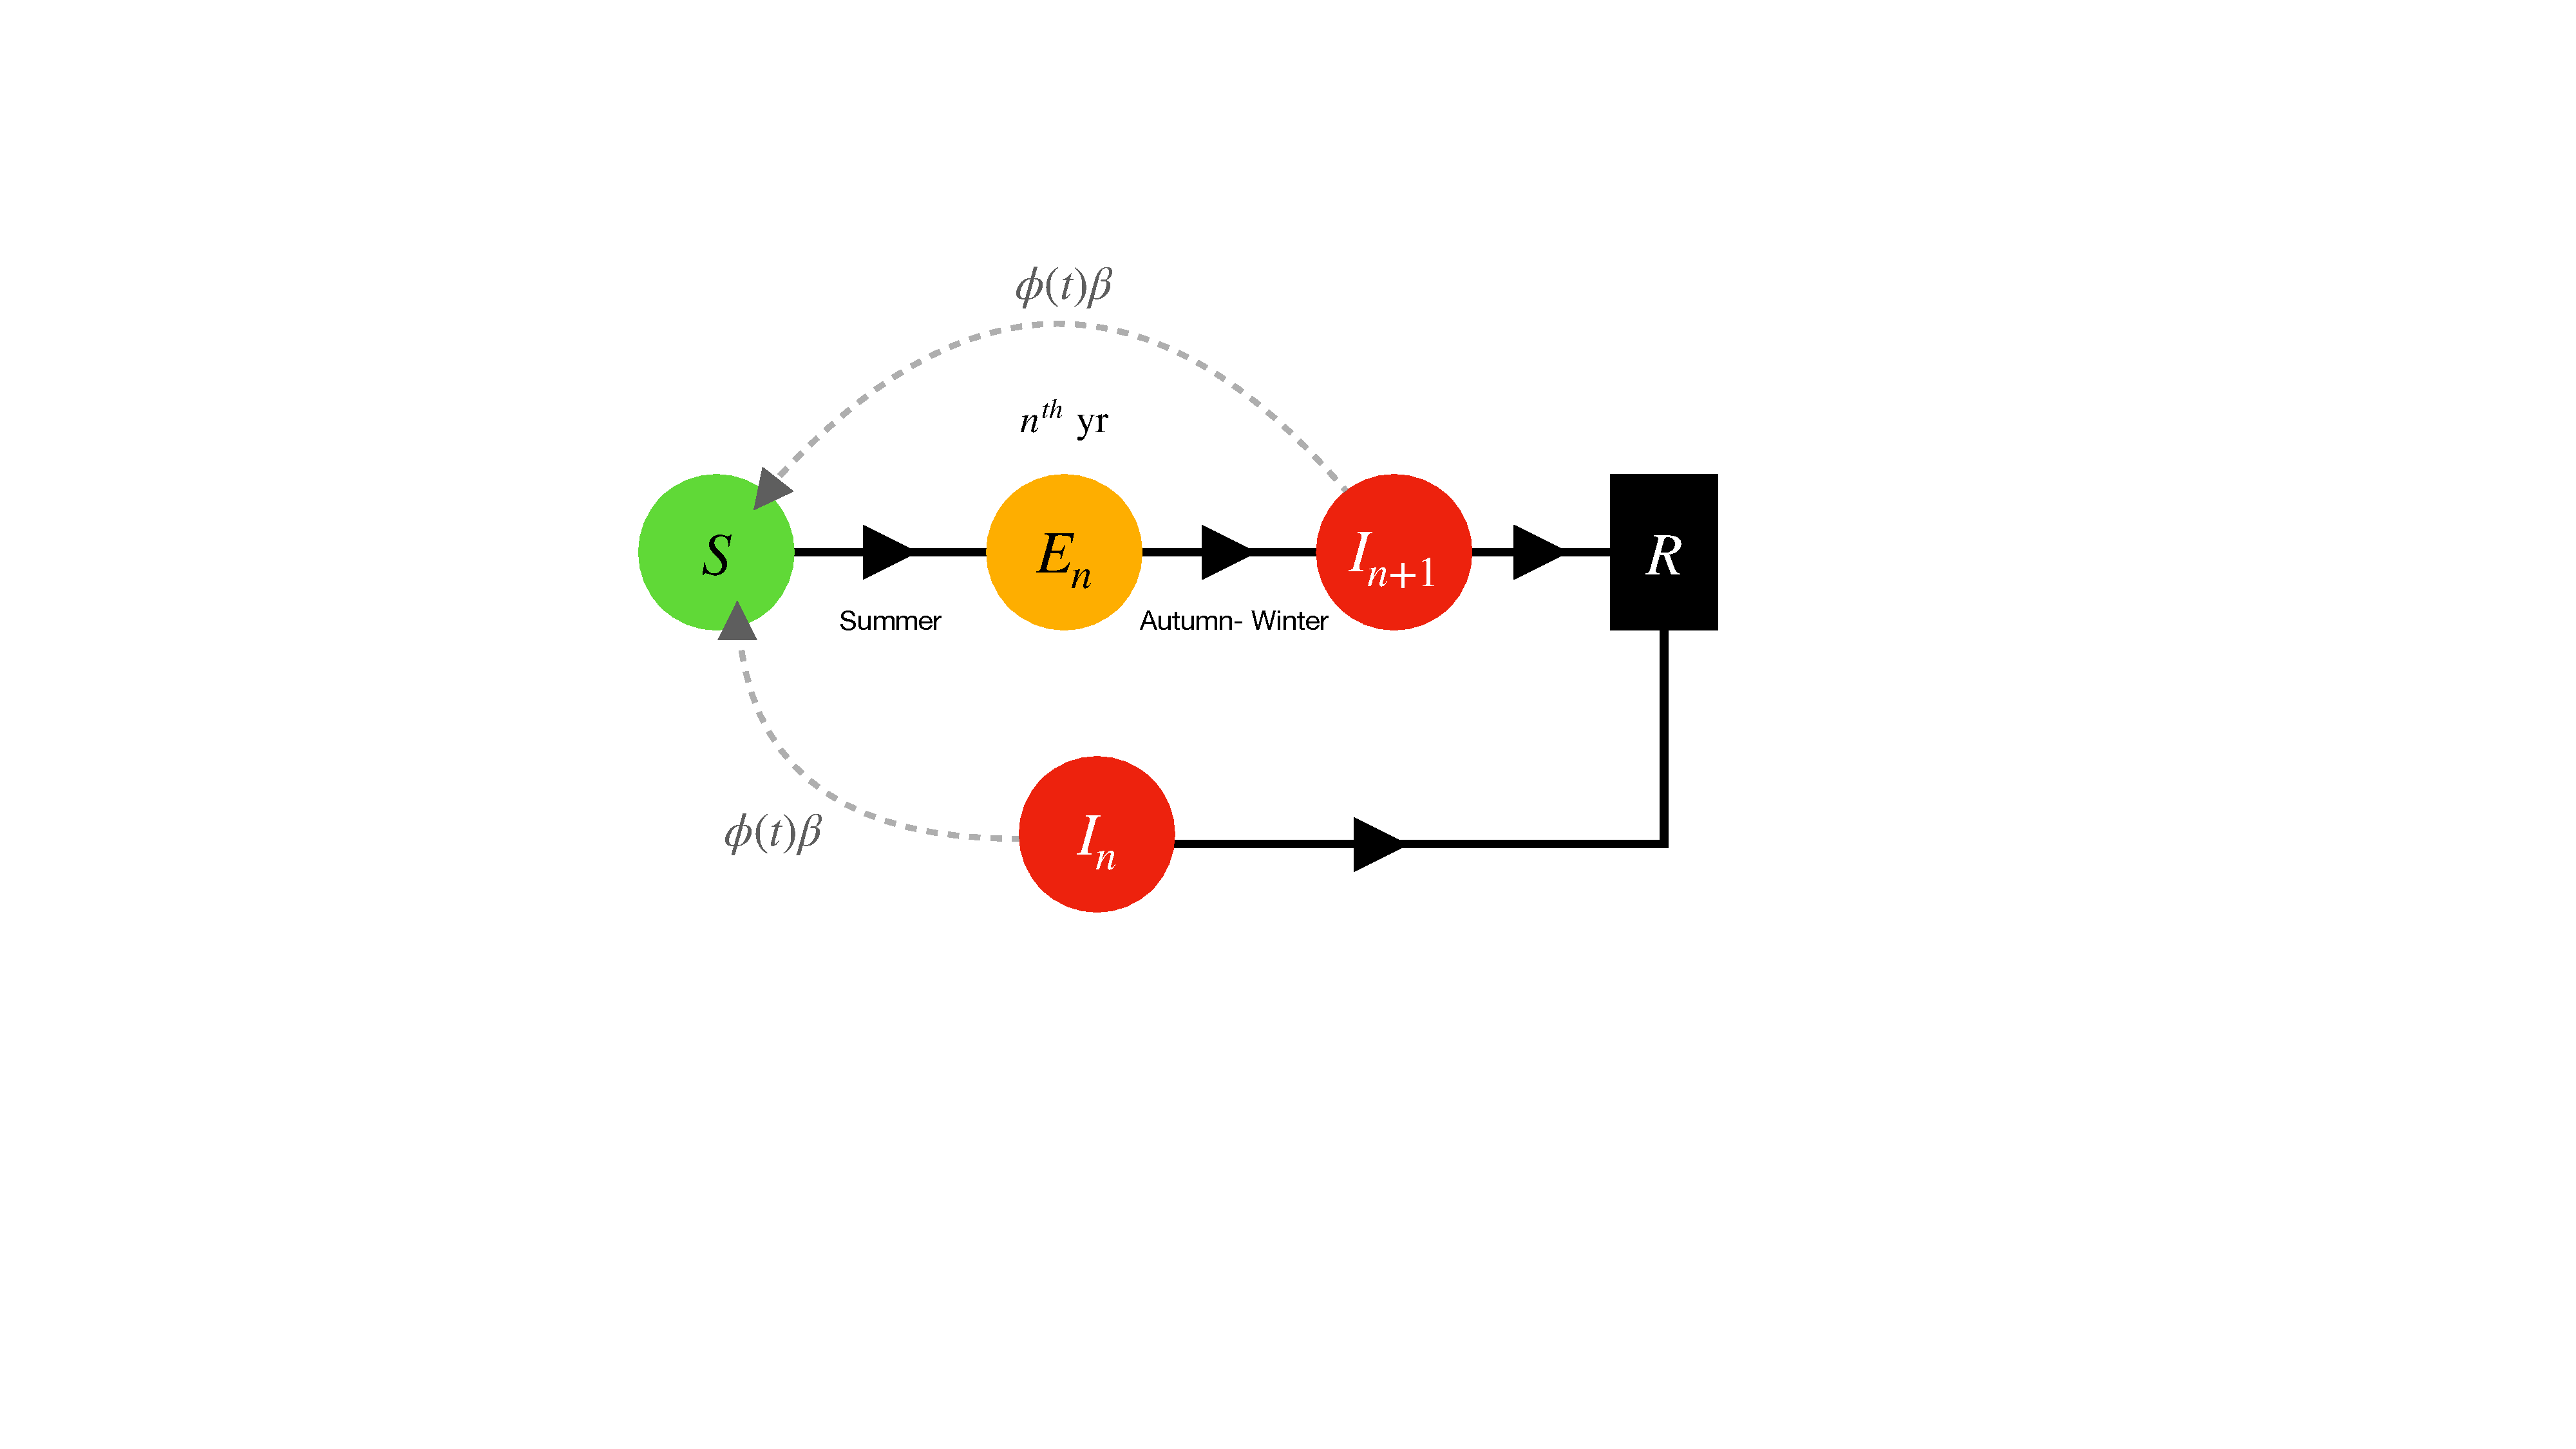
\includegraphics[scale=0.40]{chapter6/figures/fig1-seir-transitions.pdf}
    \caption{The seasonal $SEIR$ model of ADB. (a) In year $n$ of an outbreak, an infectious tree may cause a transition $S\rightarrow E_n$ during summer, depicted by the bottom dashed grey arrow. A tree that becomes latently infected in year $n$ will lead to an infectious tree in year $n+1$. Eventually, all infected ash are removed without the possibility of recovery. (b) The yearly cycle of the pathosystem ADB. Leaf-flush coincides with the sporulation season. Sporulating fruiting bodies release ascospores between June-September. Ash shedding takes place from late summer-early winter. }
    \label{fig:SEIR-transitions}
\end{figure}

\subsection{Infection dynamics}
\label{sec:infection-dynamics}

The infection dynamic comprises four states: susceptible $S$, latently infected $E$, infectious $I$ and removed $R$, and transitions occur through $S\rightarrow E \rightarrow I \rightarrow R$, without the possibility of recovery. 
Figure \ref{fig:SEIR-transitions} shows a typical scenario, an infected ash tree in the $n^{th}$ cycle (or equivalently $n$ years after the initial outbreak) may infect ash in the $S$ compartment. Newly infected ash will transition into the $n^{th}$ $E$ compartment, denoted by $E_n$, and become infectious in the following year $I_{n+1}$.

The distribution of susceptible ash is initialised by a Bernoulli trial with probability $\rho$, according to a binomial distribution.
Thus, interactions between individual hosts is modelled over a flat and randomly distributed population.
The probability $\rho$ defines the host density inside a square domain of size $\mathcal{L}$. 

Each lattice point in the $L\times L$ domain is chosen to represent a $5\mathrm{m}\times5\mathrm{m}$ patch of land that approximates the canopy cover of an average ash tree\textemdash although young saplings typically assume less area. 
A domain resolution of $5\mathrm{m}\times5\mathrm{m}$ yields an upper bound of $400$ ash trees per hectare of canopy cover, indicative of some densely populated ash stands \cite{ash-tree2, ash-tree1}. % CHECK!

\subsubsection{Transitions: $S\rightarrow E_n$}

Individual tree-to-tree interactions are modelled as a system of particles\textemdash discussed in chapter \ref{ch5:dispersal-model}.
Transitions from $S$ to $E$ involve two components: a time-varying infectivity $\beta\phi(t)\in [0, 1]$ and dispersal function $D(x,x^\prime; \ell)\in [0, 1]$.
To model dispersal, a thin-tailed Gaussian was considered alongside a normalisable fat-tailed inverse power law distribution.

In year $n$, ash located at position $x$ may transition into the exposed category under the influence of infected ash located at $x^\prime$, denoted by $S_x \rightarrow E_{x,n}; I_{x^\prime, n}$.
The probability of transition follows:
\begin{equation}
    Pr(S_{x} \rightarrow E_{x,n} ;\ I_{x^{\prime}, n} ) = \beta  \phi(t) D(x, x^{\prime}; \ell)
\end{equation}
where $\phi(t)$ is a time-dependant function reflecting the seasonal life-cycle of ADB and $r$ is the distance between $x$ and $x^\prime$.
The probability of transition is calculated for each susceptible tree in the domain (i.e. $\forall S_x \in [L, L]$),
and repeated for all infectious trees in $I_n$.
Transition probabilities are calculated at each time-step, taken to be days, while trees are infectious.
From a computational perspective, the probability of transition is assessed against samples drawn from a continuous uniform distribution $U(0, 1)$;
see Appendix \ref{a:probablity-transition} for an example of implementation.

\begin{landscape}

\begin{figure}
    \centering
    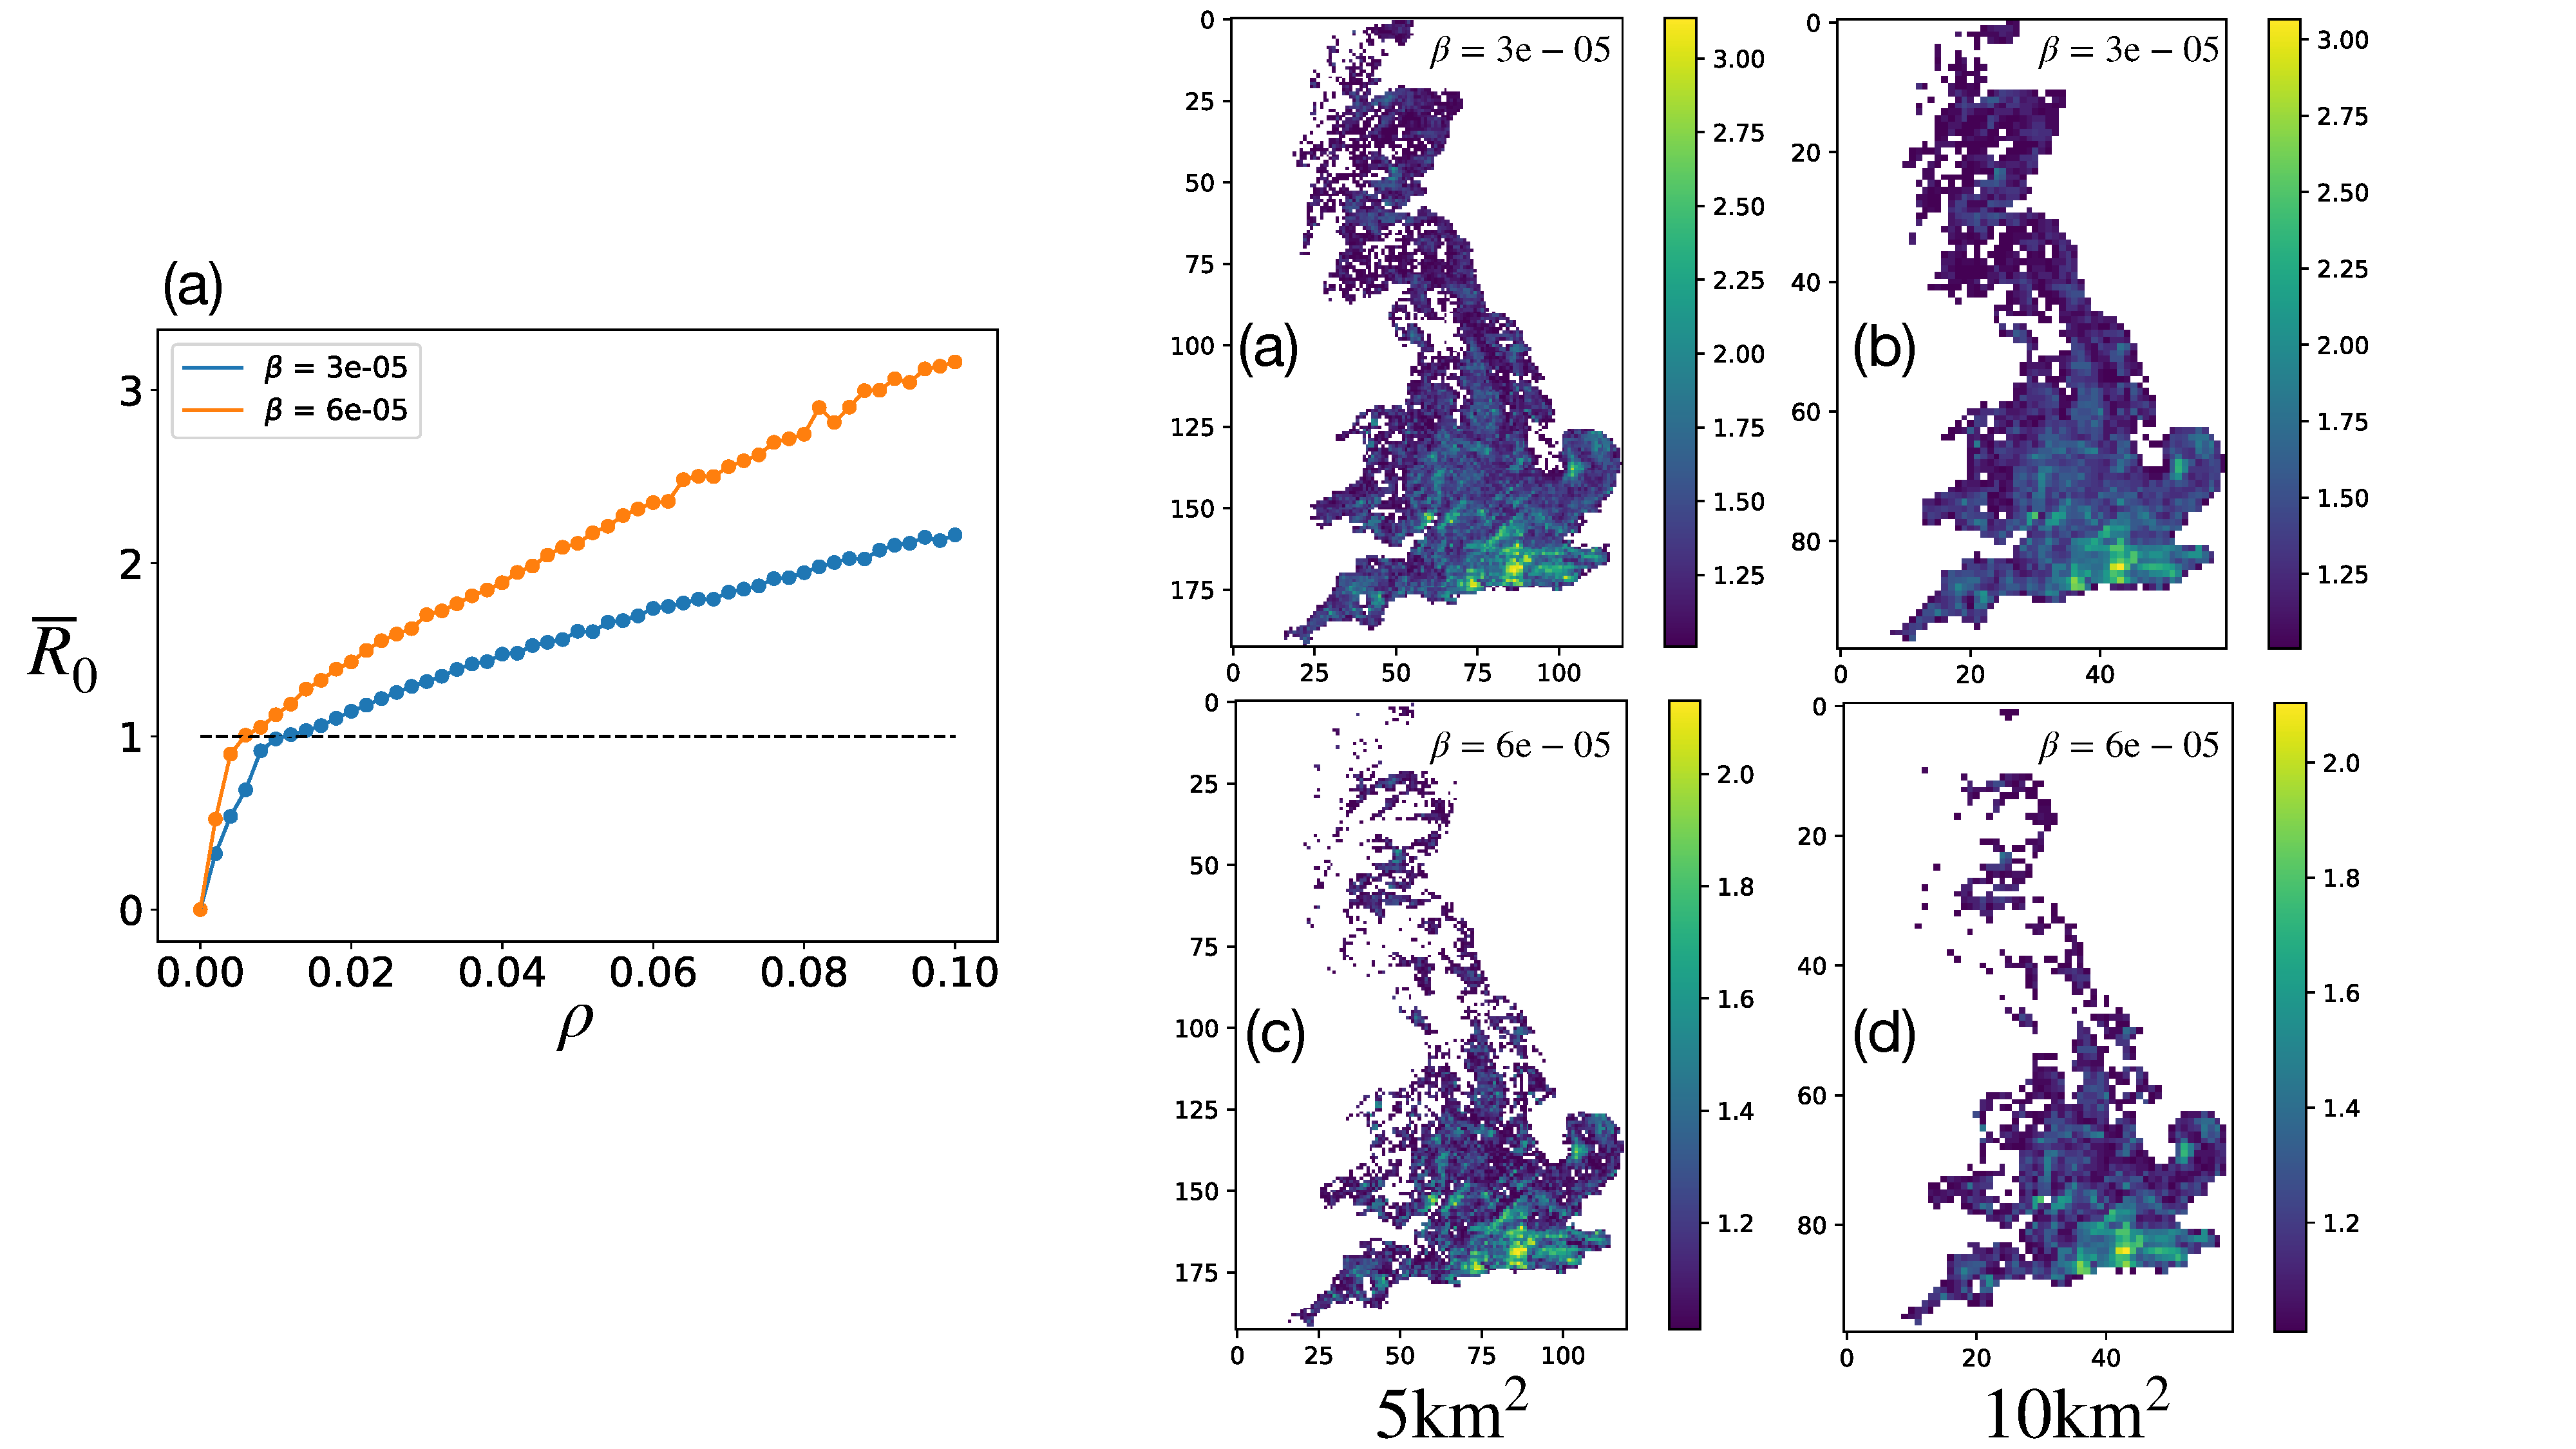
\includegraphics[scale=0.20]{chapter6/figures/fig2.pdf}
    \caption{Dispersal gradients at the local spatial scale, parameters are informed by the work of \cite{grosdidier2018tracking}. The authors provide estimates for Gaussian and inverse power law kernels: $\ell_{ga} = 195\mathrm{m}$ and ($\ell_{pl} = 205\mathrm{m}$, $a=3.3$) respectively, where $a$ represents the inverse power law exponent.}
    \label{fig:dispersal-parameterisation}
\end{figure}

\centering
\begin{table}[]
\begin{tabular}{ | p{1.5cm} | p{5.0cm} | p{5.5cm} | p{3cm} | }
\hline
 \multicolumn{4}{|c|}{Infection models $Pr(S_{x} \rightarrow E_{x,n}; I_{x^{\prime}})$} \\
 \hline
 Model & Dispersal function $D \in [0, 1]$ & Sporulation function $ \phi \in [0, 1]$ & infectivity $\beta$ \\
 \hline
 1: ga-$\phi_1$ & $D_1(x, x^{\prime}) = \exp\Big[\frac{-r^2}{2\ell^2_{ga}}\Big]$ & $\phi_1(t) = 
\begin{array}{cc}
  \{ & 
    \begin{array}{cc}
      1 & t\in [\mathrm{Jun},\ \mathrm{Sep}] \\
      0 &  \mathrm{elsewhere}
    \end{array}
\end{array} $ & here\\
 2: pl-$\phi_1$ & $D_2(x, x^{\prime}) = (1 - r/\ell_{pl})^{-a}$ & $\phi_1(t) = 
\begin{array}{cc}
  \{ & 
    \begin{array}{cc}
      1 & t\in [\mathrm{Jun},\ \mathrm{Sep}] \\
      0 &  \mathrm{elsewhere}
    \end{array}
\end{array} $ & here\\
 3: ga-$\phi_2$ & $D_1(x, x^{\prime}) = \exp\Big[\frac{-r^2}{2\ell^2_{ga}}\Big]$ & $\phi_2(t) = \exp\Big[-\frac{(t - T_{SP})^2}{2\sigma_{SP}^2}\Big]$ & here\\

 4: pl-$\phi_2$ & $D_2(x, x^{\prime}) = (1 - r/\ell_{pl})^{-a}$ & $\phi_2(t) = \exp\Big[-\frac{(t - T_{SP})^2}{2\sigma_{SP}^2}\Big]$ &here \\
 \hline
 \end{tabular}
  \caption{Four model variants are considered, composed of either: Gaussian (ga) or inverse power law (pl) dispersal and heavy-step ($\phi_1$) or peaked ($\phi_2$) sporulation.
The corresponding model parameters are shown below in Table \ref{tab:SEIR-model}.}
\label{tab:model-variants}
\end{table}
\end{landscape}

The sporulation function $\phi$ dictates when infectious trees in $I_n$ produce new secondary infections. 
For ADB, sexual reproduction repeats yearly from June to September during its \textit{`sporulation season'}.
As such, $\phi$ is non-zero during this period.
Specifically, two sporulation functions are considered, $\phi_1$ and $\phi_2$, based on a heavy-step and peaked normal distribution respectively.
Sporulation is the topic of section \ref{ch6:sporulation} below, alongside the precise functional form of $\phi_1$ and $\phi_2$.
Altogether there are four models, summarised in \ref{tab:model-variants}.

In the $E$ compartment, trees are infected but not infectious i.e. latently infected.
Ash infected with \textit{H. fraxineus} take approximately two weeks to display symptoms,
and start to shed infectious leaves in following autumn after infection \cite{gross2014h}.
The compartments $(E_1, E_n,..,E_n)$ represent the same biological state of latently infected.
The index $n$ is merely included for convenience to highlight the fact that in this model, it takes latently infected ash takes approximately one year to start produce new secondary infections during the $(n+1)^{th}$ sporulation peak.

% The inclusion of an exposed category, together with a sporulation function, constrain the dynamics of ADB whereby: A) infected ash may be latently infected and display symptoms but crucially not disperse any infectious material B) ash may shed infected leaves in Autumn/winter, and thereby disperse infected material, but not lead to any secondary infections until the following summer when ascospores are produced.
% in the model, and a time-dependant sporulation function $\phi$ controls infectivity of leaf-litter.

\subsubsection{Transitions: $E_n\rightarrow I_{n+1}$}

As defined here, a latently infected ash in $E_n$ transitions into the infectious compartment, $I_{n+1}$, at the fist onset of seasonal leaf shedding between autumn and winter.
Infected ash disperse infectious leaf-litter each year following infection until it's eventual demise;
this dynamic assumes that all ash are susceptible, and that leaf-infection spreads to the ash xylem with perfect fidelity. 
In reality, a variety of genetic and environmental factors influence the ability of ADB to invade an ash.
Although \textit{H. fraxineus} is able to infect ash leafs regardless of tolerance, only the minority of tolerant individuals can prevent the pathogen from invading the xylem.

A Gaussian distribution represents the onset of ash leaf-shed, and therefore the transition $E_n\rightarrow I_{n+1}$.
The Gaussian distribution was chosen to be centred in November, $T_{LS},$ with a two-week standard deviation $\sigma_{LS}$,
The normally-distributed form of leaf-shed was based on observations of leaf litter-fall rates in deciduous forest \cite{zhang2014seasonal, dixon1976analysis}, 
which typically follow peaked distributions that repeat yearly.

\begin{table}[h]
\centering
\begin{tabular}{l l l}
\hline
\textbf{Model parameter} & \textbf{Description} & \textbf{Value(s) taken}\\
\hline
$\rho$  & Tree density & $0.00 - 0.10$ \\ 
$\beta$ & Infectivity & $0 - 10^{-3}$ \\
$\ell_{ga}$ & Gaussian dispersal scale parameter& $196\mathrm{m}$ \\
$\ell_{pl}$ & inverse power dispersal law scale parameter& $203\mathrm{m}$ \\
$a$ & Inverse power law exponent & $3.3$ \\
$t$ & Time-step & $1\ \mathrm{day}$\\
$T$ & Sporulation season & June - September \\
$T_{SP}$ & Peak sporulation $\phi_2$ & end of July \\
$T_{LS}$ & Peak ash leaf-shedding & mid-November \\
$\sigma_{LF}$ & Leaf-shedding standard deviations & 2 weeks \\
$\alpha$ & Lattice constant & $5\mathrm{m}$ \\
$\mathcal{L}$ & Square lattice dimension & $200$ - $2000$ \\
$A$ & Domain area & $1\mathrm{km^2}$ - $20\mathrm{km^2}$ \\
$\lambda$ & Mean infectious life-time & $5\ \mathrm{years}$ \\
$R_0$ & Mean reproduction number & $0-20$ \\
\hline
\end{tabular}
\caption{Parameters used in the $SEIR$ model of ash dieback. The dispersal parameters are taken from \cite{grosdidier2018tracking} and the typical tree densities of ash are informed from by \cite{hill.data}.}
\label{tab:SEIR-model}
\end{table}

Centering the normal distribution in mid-November, with a two-week standard deviation ensures that the earliest possible onset of leaf-shed (described by the left-hand tail) begins in the month of September.
In the field, the timing of ash shedding their leaves is more complicated and thought to be dependant on tree age. 
Observations by \cite{hietala2013invasive} suggest that younger ash begin to defoliate in late August, while large dominant ash begin to shed in early October.

To my knowledge, litter-fall rates for ash have not been calculated,
so choosing a normal distribution centered in mid-November with a two-week standard deviation is ultimately ill-informed. 
However, time delay between the transition $E_n \rightarrow I_{n+1}$ in autumn/winter and the sporulation function $\phi(t)$ becoming sufficiently large in summer affords some degree of flexibility in the exact time-scale.
From a mathematical standpoint, provided that latently infected ash transition into the infected compartment before the sporulation season, 
the epidemic spread in this model will remain the same
\footnote{The seasonal pattern of litter-fall is an important factor to consider in ecosystem function and forest health and has been well-researched. 
A more complex model of ADB, involving soil-borne interactions, could incorporate the build up infected leaf biomass into a time-varying $\beta$. 
However, it remains to be seen if this is necessary to capture the essential dynamics of wind-borne dispersal.}. 

\subsubsection{Transitions: $I_n\rightarrow R$}

The last transition to consider is from infected to removed $I_{n}\rightarrow R$. Given a $95\%$ mortality rate, ADB can be regarded as lethal \cite{ash-dieback-costs}.
Therefore, once an ash tree becomes infected, an eventual transition to the $R$ compartment is assumed with certainty.
As mentioned above, the picture is more complex in reality. 
For example, stress-free trees in urban settings can survive for long periods of time if pruned, and the low minority of healthy tolerant trees can fight off the infection.
Additionally, other rare edge-cases can contradict this assumption;
laboratory experiments have shown that after a \textit{`massive ascospore inoculation'}, leaf-shed can result before the infection has the chance to spread throughout the tree \cite{https://doi.org/10.1111/mpp.12073}.

Ash dieback effects trees of all ages with younger ash being more susceptible and larger, mature ash being more tolerant. 
As a first approximation, infected ash were chosen to have exponentially distributed life-times with a mean of five years, see table \ref{tab:SEIR-model}.
This choice was informed by experimental observations of ash mortality after years of infection. 
In particular, reports of $5\%$ mortality after two years of infection \cite{kessler2012dieback}, $75\%$ mortality within five years \cite{langer2015ash}  % Brush up in relation t age classes
and no observations of infected ash surviving beyond $15$ years \cite{wylder2018evidence} provide some guidance towards an approximate time-scale.
The precise probability distribution describing $I_{n}\rightarrow R$ is, to my knowledge, non-existent in the literature. 

\subsection{Dispersal parameterisation}

Dispersal was informed by data collected in France by \cite{grosdidier2018tracking}. The field study conducted by \cite{grosdidier2018tracking} provide estimates for dispersal parameters by fitting data against a Gaussian and inverse power law kernels. Notably, the authors studied dispersal at two different spatial scales, local and regional, \textcolor{red}{on the order of $1\mathrm{km}$, to $10-100 \mathrm{km}$ respectively}. For a review on the importance of scale, see chapter \ref{chapter2:litreview}. 

The experimental data analysed by \cite{grosdidier2018tracking} tracked ADB spores about known sources of infection. Although data on spore depositions does not necessarily correspond to a new infection, it sheds essential light on the spatial scale of ADB dispersal. Given that the spatial scale in the $SEIR$ model is small, at a  resolution of $5\mathrm{m} \times 5\mathrm{m}$, a decision was made to parameterise dispersal with the local-level dispersal values given by \cite{grosdidier2018tracking}. See table \ref{tab:SEIR-model} an Fig\ref{fig:dispersal-parameterisation}. 

The decision to use ADB scale parameters given by \cite{grosdidier2018tracking} suppose that the spread of ADB in Great Britain is comparative to the spread of ADB in France. Nonetheless, there is a noticeable difference in the French climate, landscape and, importantly, wind patterns. % references
Notwithstanding these differences, it stands to reason that dispersal parameters, if measured over a smaller, local spatial scale, would be less pronounced. 

Lastly, the regional-scale dispersal analysed by \cite{grosdidier2018tracking}, measured over spatial scales of $10$-$100\ \mathrm{km}$, is thought to contain artefacts of LDD by human-mediated transport. The regional spread of ADB though LDD is, therefore, beyond the scope of the present chapter\textemdash a discussion of LDD will conclude this chapter and lead us to chapter into chapter \ref{ch7:pde}.


% Q: what is the relationship between the mortality ratio (or final fraction of infected hosts) ? 
% If R0 was considered over a larger time-scale, host-regrowth would need to be integrated into the model
% Furthermore, measuring R0 over a larger time-scale could over, or underestimate, the degree to which a response would need to be undertaken in the response time-window. 
% a basic reproduction number $R_0$ is defined for the first life-cycle of the pathogen.
% Moreover, data over a relatively short time scale is typically all that is available when making decisions about control, not to mention the added complexity of incorporating host-regrowth–which becomes an important factor over longer time scales–and so, the constraint of computing R0 over longer time scales is relaxed. 
%  We develop the simplest implementation possible, namely, where R_0 is measured over one pathogen life-cycle, and the course of infection for each host follows the same process with perfect fidelity. This lies in stark contrast to a realistic scenario whereby different hosts show considerable differences.

% \begin{itemize}
%     \item see for a review on how R0 is calculated \cite{perspectives-on-r0}, we use method x in order to estimate and inform R0
%     \item $R_0$ is a complex function which changes in time, to this end, the next generation operator is used to derive a value for $R_0$ \cite{doi:10.1098/rsif.2009.0386}. In order to inform the value of $R_0$ we do xy and
%     \item Although it is hard to enforce a true $R_0$ value, the most important feature introduced from the definition is a threshold from which we can see if a local invasion is likely to take place.
%     \item Since the number of susceptible hosts is fixed, without replacement, the number of susceptible hosts will continually decrease in time in the case of an epidemic. Given the strong spatial component in the model we expect that measuring $R_0$ as-per this definition will give an under-estimate for later times when few susceptible trees remain. Likewise, for earlier times when susceptible neighbours are plentiful $R_0$ will yield an upper estimate for the pathogen. In order to characterise the pathogen in this model, we take the upper bound defined between the $1^{st}-2^{nd}$ generations. This simplification represents a worst-case scenario and the mean value of $R_0$ would be lower for later times when there are less trees available to infect. But most importantly, the threshold of transmission $R_0>1$ is reliable captured \textit{during the initial stage of infection}.
%     \item $R_0$ can be fully characterised by a growth rate \cite{R0-construct}. That is, the growth factor per generation.
% \end{itemize}

\section{Seasonal $SEIR$ model behaviour}

Previously in section \ref{sec:infection-dynamics} the details of sporulation were omitted. For robustness, two sporulation functions are considered, a step function defined by equation \ref{eq:step-function} and a normal distribution located at the midpoint between June and September. For now, the simplest form of sporulation is adopted: % DISCUSS PLANK SPORULATION...
\begin{equation}
\label{eq:step-function}
\phi_1(t) = 
\begin{array}{cc}
  \{ & 
    \begin{array}{cc}
      1 & t\in [\mathrm{June},\ \mathrm{September}] \\
      0 &  \mathrm{elsewhere}
    \end{array}
\end{array}
\end{equation}

The $SEIR$ model behaviour is shown in Figure \ref{fig:SEIR-spread} for the inverse power law dispersal model over the average density of ash in Great Britain.
The Gaussian-based dispersal model displays the same seasonal behaviour, as demonstrated in appendix \ref{section:ga-SEIR-variant}. For each year after outbreak, a rise in the number of latently infected ash in $E$ can be seen during summertime sporulation, June-September, followed by a rise in the number of infectious ash in the Autumn-Winter. 

The spatial progression of ADB in the $SEIR$ model is shown in Figures \ref{fig:SEIR-spread}(a-c) over one year. The simulation begins in Figure \ref{fig:SEIR-spread}(a) with an initial condition of $25$ infected ash distributed throughout the host landscape during March. At this point in the year, fungal fruiting bodies on infected leaf litter will be preparing to release ascospores.
During the sporulation season, secondary infections are produced, and latently infected ash spread throughout the domain, depicted by the orange dots in Figure \ref{fig:SEIR-spread}(b). After the sporulation season ends in September, latently infected ash begin to transition into the $I$ compartment, reflected by the increased number of red dots in Figure \ref{fig:SEIR-spread}(c). The cycle will continue when the next cohort of secondary infections are produced in the following summer when the sporulation function next becomes non-zero.

The number of ash in the $SEIR$ compartments (on logarithmic axes) is shown in Figure \ref{fig:SEIR-spread} for three infectivity parameters in a $2\mathrm{km}\times2\mathrm{km}$ domain. Figure \ref{fig:SEIR-spread} shows three scenarios over $10$ years with infectivity parameters $\beta \in [2.5\times 10 ^{-4}, 1.5\times 10 ^{-4}, 1.5\times 10 ^{-5}]$, above, around and below the epidemic threshold, (d-f) respectively. In Figure \ref{fig:SEIR-spread}(d), $\beta$ is above the epidemic threshold and the number of ash in $S$ decline rapidly, shown by the blue line. During seasonal sporulation, large spikes in the number of latently infected ash can be seen in orange. Latently infected ash quickly transition into $I$ during Autumn and winter, as shown by the seasonal rise of $I$ in green.

\begin{landscape}
\begin{figure}
    \centering
    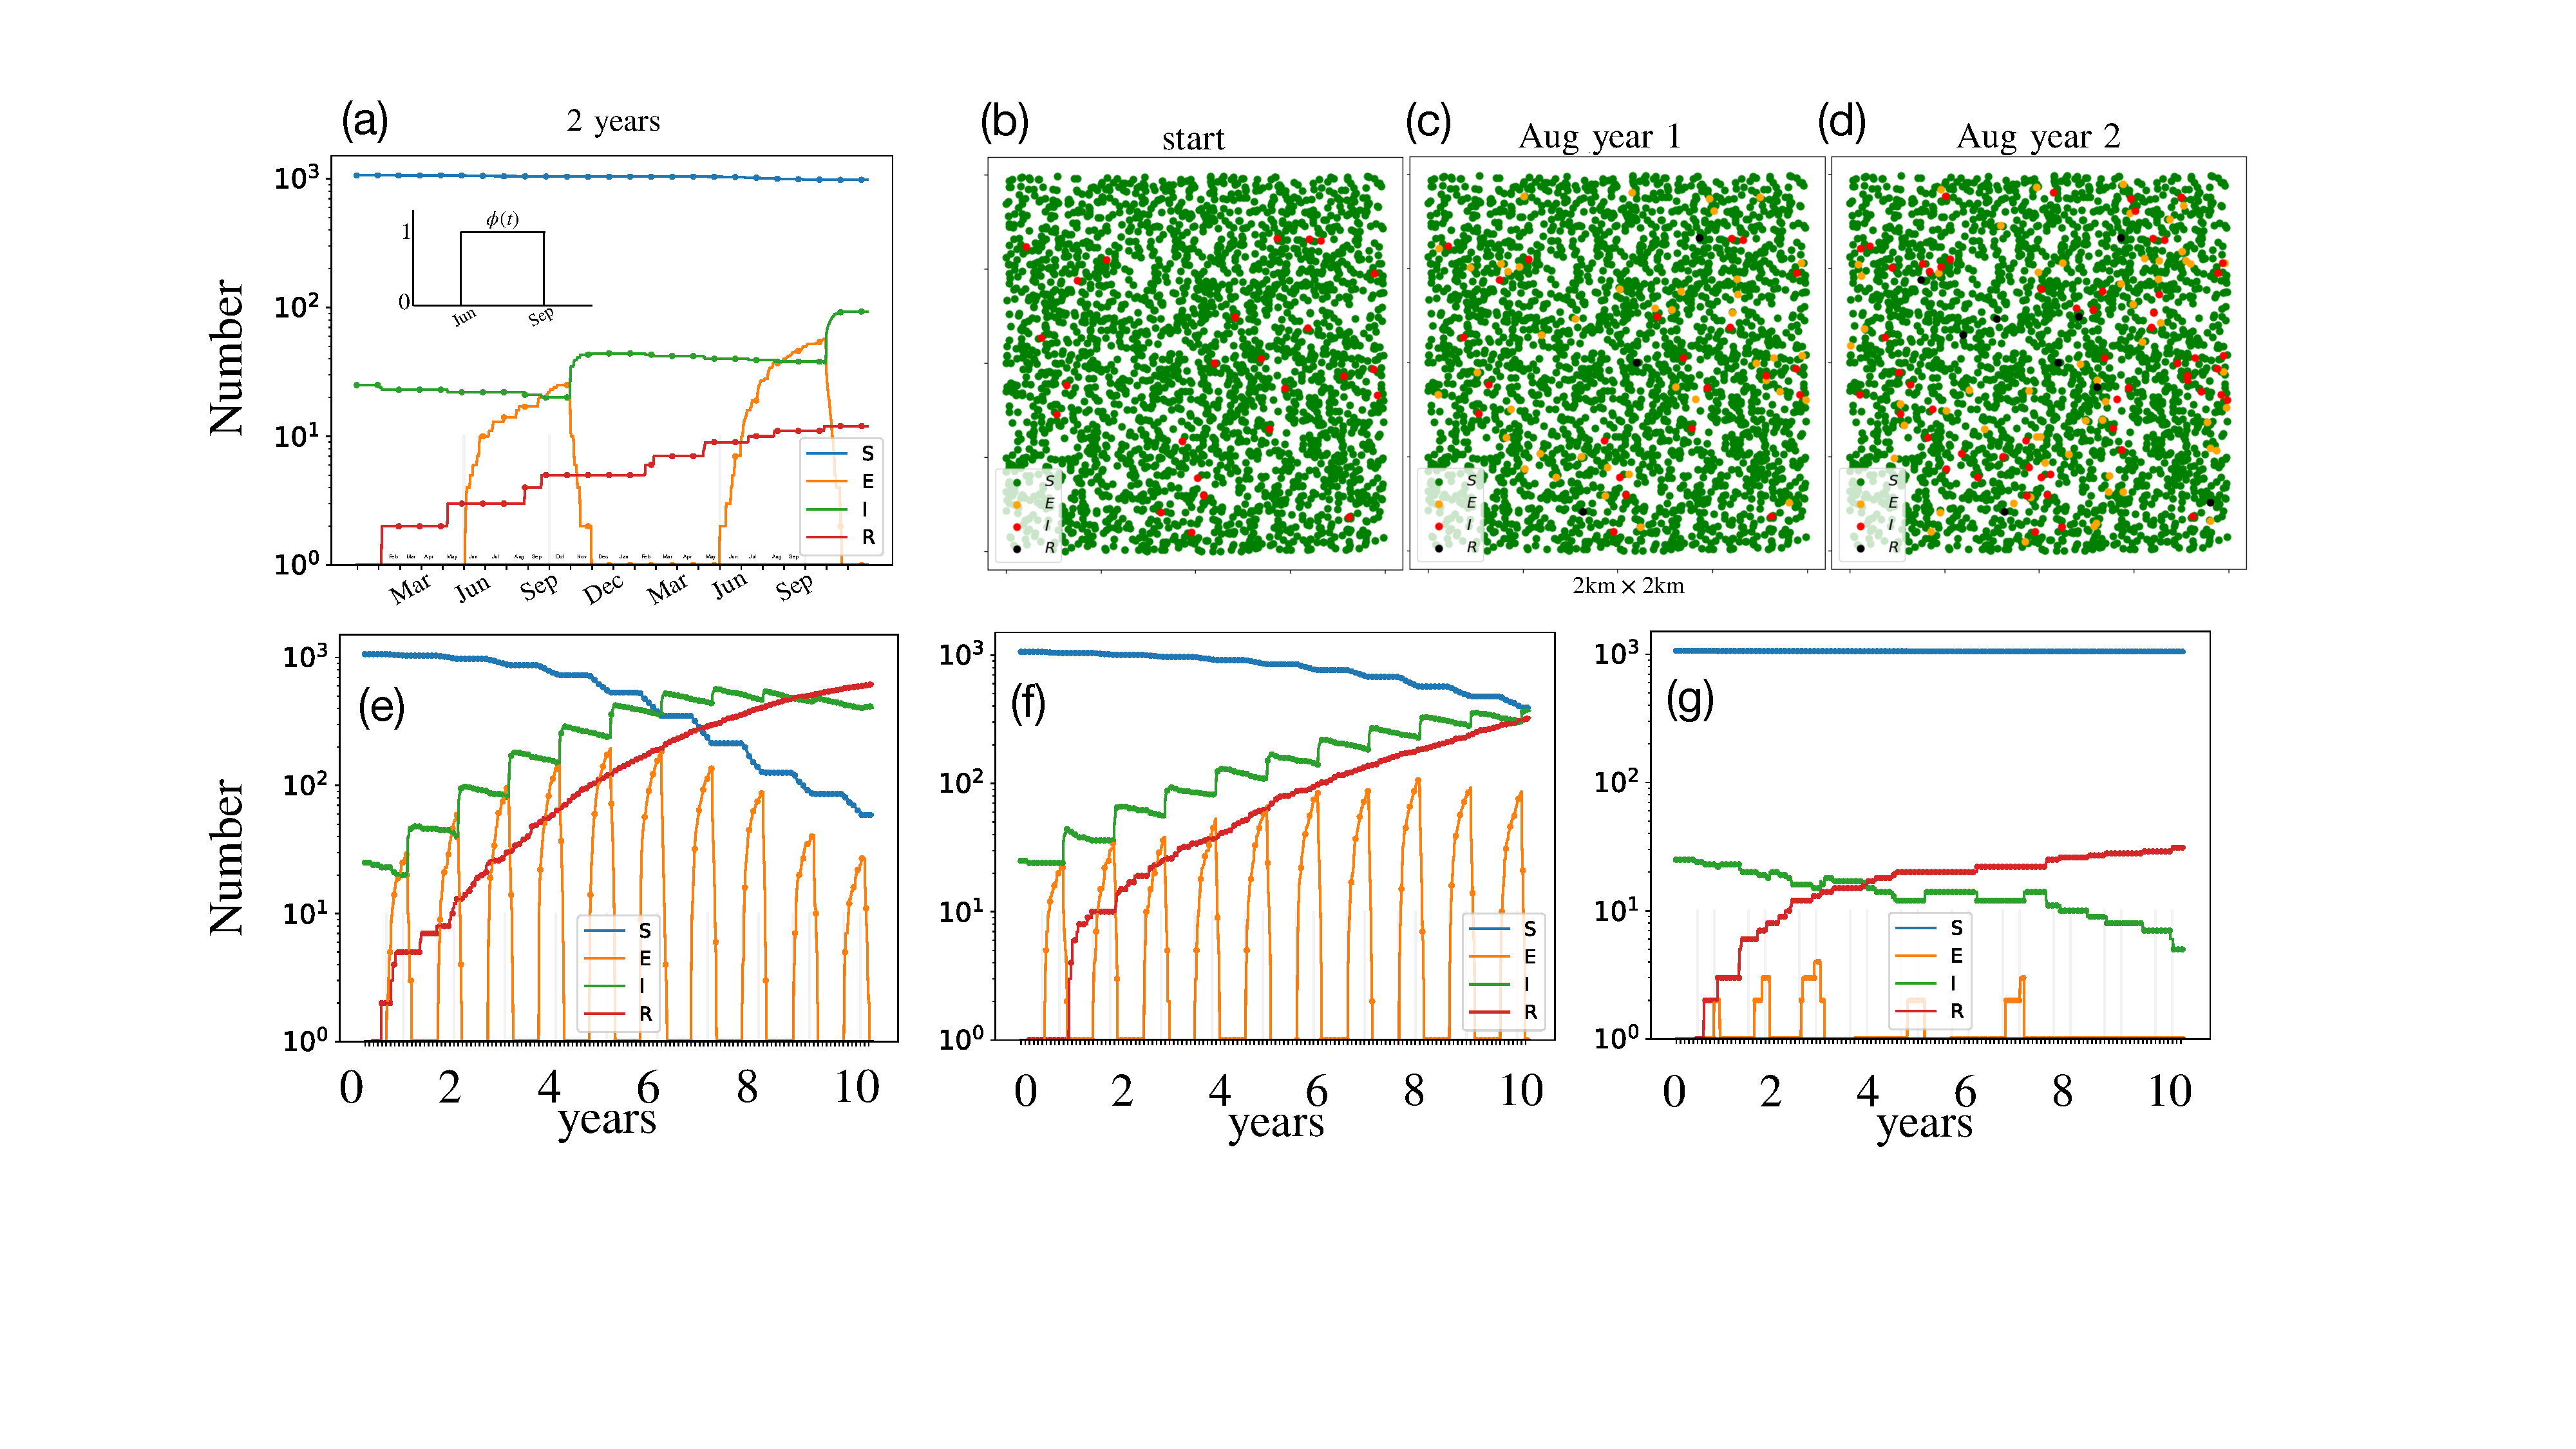
\includegraphics[scale=0.45]{chapter6/figures/fig4-seir.pdf}
     \caption{The inverse power law $SEIR$ model of ADB shown over the average ash density $\overline{\rho} = 0.017$. (a-c) The spatial progression of disease in a $2\mathrm{km} \times 2\mathrm{km}$ domain over one sporulation season beginning with $25$ infected ash distributed throughout the domain. (d-f) The number of ash in the $SEIR$ compartments are shown over ten years for infectivity parameters above, around and below the epidemic threshold respectively.}
    \label{fig:SEIR-spread}
\end{figure}
\end{landscape}

In Figure \ref{fig:SEIR-spread}(e) infectivity parameters are slightly above the epidemic threshold and the model behaviour is similar, albeit with a slower seasonal decline and rise in $S$ and $I$. For infectivity parameters below the epidemic threshold, Figure \ref{fig:SEIR-spread}(f), $S$ remains approximately constant and $I$ slowly declines. Interestingly, Figure \ref{fig:SEIR-spread}(f) persistence in model of ADB; whereby, even if the epidemic parameters are below the threshold, the fungus may survive for long periods of time. In general, persistence in plant-based pathogens is one aspect that complicates epidemic control\textemdash see chapter \ref{ch3:invasions_and_persistence} for a review of invasion and persistence in the spread of plant-based diseases

\subsection{Sporulation: time-varying infectivity}
\label{ch6:sporulation}

Time varying infectivity rates are an important concept in epidemiology, this is true of epidemics in both human/animal \cite{svensson2007note, liu2012infectious} 
and botanical populations \cite{suffert2018some, leclerc2014estimating, time-varying-infectivity} and in particular, ADB \cite{grosdidier2018tracking, hietala2013invasive}. 
The life-cycle of ADB is highly time-dependant. The peak of ADB infectivity occurs during summertime sporulation, when fruiting bodies on dead litterfall release ascospores.
Two sporulation functions, $\phi_1(t)$ and $\phi_2(t)$ are used to model the reproductive life-cycle and infectivity of ADB.
The result of multiply the infectivity parameter with sporulation, $\beta\phi(t)$, is a representation of time-varying infectivity. 
In a more complex model, $\phi_1(t)$ and $\phi_2(t)$ would represent the number of spores produced by infected litterfall. In the model of ADB presented here, $\phi(t)$ is dimensionless and serves only to capture the time-variation of infectivity.

Due to the seasonality and perennial nature of ADB, both $\phi_1(t)$ and $\phi_2(t)$ repeat yearly, becoming non-zero during the months of June and September
\footnote{Variations in ADB sporulation have been noted between European countries \cite{https://doi.org/10.1111/mpp.12073}, along with the potential for early-onset sporulation in the face of favourable environmental conditions. Although, the most generally agreed upon sporulation period is thought to be from June to September.}.
To inform sporulation functions, we draw on the modelling work of \cite{time-varying-infectivity} and \cite{segarra2001epidemic}
\textemdash these studies are reviewed in chapter \ref{ch2:lit-rev-compartmentalised-models}. 
Both models of sporulation are shown in the insets of Figures \ref{fig:SEIR-sporulation}(a-b), that is, a step and Gaussian function respectively. 

Here, the function $\phi_2(t)$ is a special case of the Gamma(k) presented in \cite{time-varying-infectivity, segarra2001epidemic} and can be described by:
\begin{equation}
\label{eq:step-function}
\phi_2(t) = 
\begin{array}{cc}
  \{ & 
    \begin{array}{cc}
      \exp(-\frac{(t - T_{sp})^2}{2\sigma_{sp}^2}) & t \in[\mathrm{June}, \mathrm{September}] \\
      0 & \mathrm{elsewhere}
    \end{array}
\end{array}
\end{equation}
where $T_{sp}$ is taken to be the mid-point of June-September (i.e. late July/early August) and $\sigma_{sp}^2$ is a standard deviation of two weeks. As discussed above, the choice of standard deviation informs the earliest transitions from $S\rightarrow E$, based on observations from \cite{grosdidier2018tracking, hietala2013invasive}. 

In the insets of Figure \ref{fig:SEIR-sporulation}(b), $\phi_2(t)$ approaches zero as $t$ approaches the months of June and September; the likelihood of new secondary infections at these points in time is therefore low. However, to prevent the unlikely scenario of new secondary infections occurring before and after the sporulation season, $\phi_2(t)$ was effectively multiplied by the step function $\phi_1(t)$, assuring the impossibility of secondary infections outside of the sporulation season.

The behaviour of both models over two years is shown in Figure \ref{fig:SEIR-sporulation}. Both models show a rise in the number of infected ash during the sporulation, albeit with different values of $\beta$.
The peak in $\phi_2$ leads to a rise in the number of new secondary infections in July, slightly later in the year compared to $\phi_1(t)$. The sporulation function $\phi_2(t)$ also requires a higher value of infectivity $\beta$ to generate the same level of epidemic impact; this can be understood by the smaller area under the curve of $\phi_2(t)$, shown in the insets of Figures \ref{fig:SEIR-sporulation}(a-b). 

\begin{figure}
    \centering
    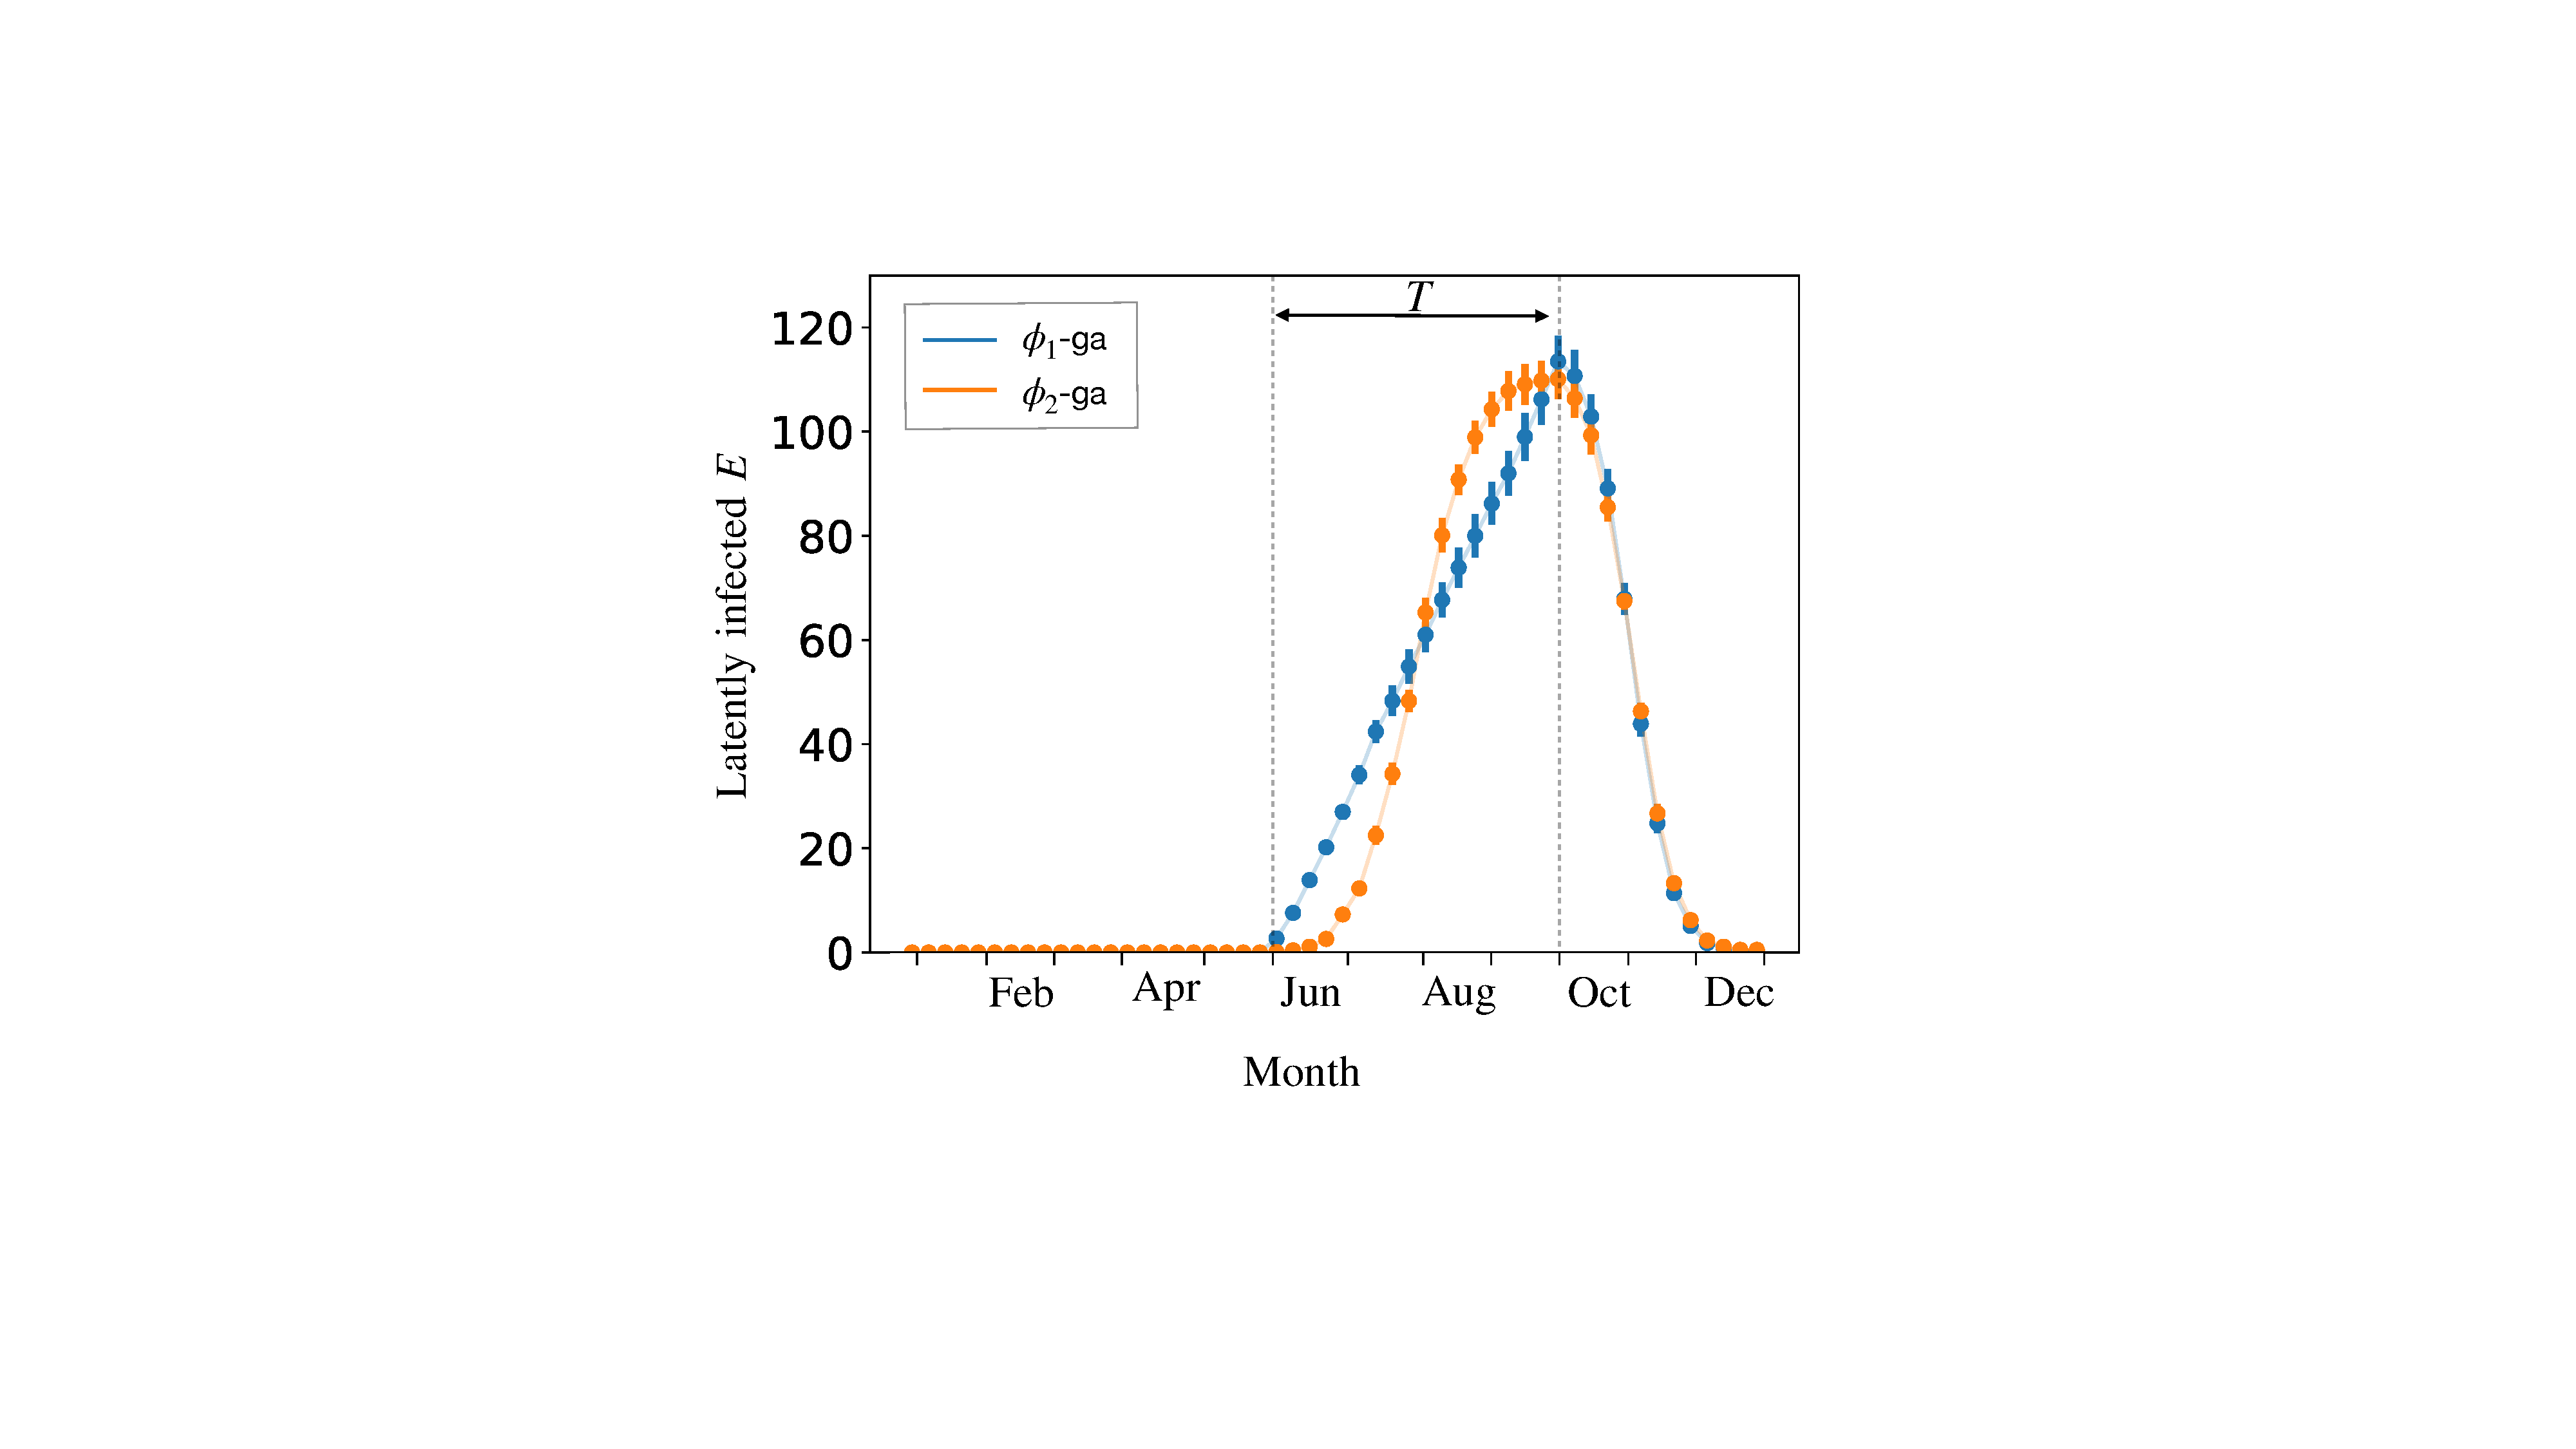
\includegraphics[scale=0.45]{chapter6/figures/fig5-sporulation.pdf}
    \caption{Two year simulations of the power law dispersal model are shown for the sporulation functions $\phi_1(t)$ and $\phi_2(t)$, (a) and (b) respectively.}
    \label{fig:SEIR-sporulation}
\end{figure}

During sporulation, the infectivity time-dependence is not uniform. Observations by \cite{hietala2013invasive} and \cite{grosdidier2018tracking} suggest that the release of ascospores peaks in mid-July to mid-August; this motivated the inclusion of $\phi_2(t)$. Despite the differences in $\phi_1$ and $\phi_2$, the model behaviour looked similar under a different scaling of $\beta$.
The difference in epidemic impact between sporulation models could be offset by normalising both distributions, as done in \cite{time-varying-infectivity, segarra2001epidemic}. 
Although, in this model of $ADB$, $\beta$ is the free parameter that would be used to fit model behaviour to data. In this interpretation, differences between sporulation models can be absorbed by re-scaling $\beta$ accordingly.

\section{Defining an $R_0$}

Before the $SEIR$ model can be investigated, a measure of the pathogens ability to invade must be defined. For epidemic systems, this usually comes in the form of a reproduction number $R_0$. There are, however, various challenges involved in defining $R_0$ when there are dispersal-mediated secondary infections and spatial structure, as explored in chapter \ref{ch5:dispersal-model}. Chapter \ref{ch5:dispersal-model} demonstrated that $R_0$ is a spatiotemporal function of various epidemiological parameters, and measuring $R_0$ over different spatiotemporal scales can lead to different, and sometimes misleading, results for $R_0$; for a seasonal-based pathogen such as ADB, additional factors only complicate the definition. 

\textit{From this point on, unless otherwise sated, the method for calculating $R_0$ will refer to the average number contact traced secondary infections for each generation of infection, as per Definition \ref{def:R0_contact_traced}. However, this time, secondary infections characterise the transition $S\rightarrow E$ and successive generations of infected ash arise seasonally during sporulation.}

As demonstrated in chapter \ref{ch5:dispersal-model}, a suitable spatial and temporal scale must be chosen to measure $R_0$. Figure \ref{fig:SEIR-R0-definition} shows the contact-traced $R_0$ for the inverse power law model $SEIR$ spreading above the threshold\footnote{The Gaussian variant of the $SEIR$ model also follows the same characteristic decline in $R_0$ for each subsequent generation, as demonstrated in chapter \ref{ch5:dispersal-model}}. For the particular combination of pathogen parameters shown in Figure \ref{fig:SEIR-R0-definition}(a), $R_0$ saturates to around $4$ and there is little difference in measuring $R_0$ between $10, 15$ and $20$ years. Although, measuring $R_0$ over a five year is slightly below the $10-20$ year average. This behaviour is also reflected in Figure \ref{fig:SEIR-R0-definition}(b) where $R_0$ for the first generation infected ash saturates at around $R_0 = 4$. On average, we would expect to see more infectious pathogens saturate faster and less infectious pathogens take longer\textemdash see Appendix \ref{fig:a-R0-saturate}.

\begin{figure}
    \centering
    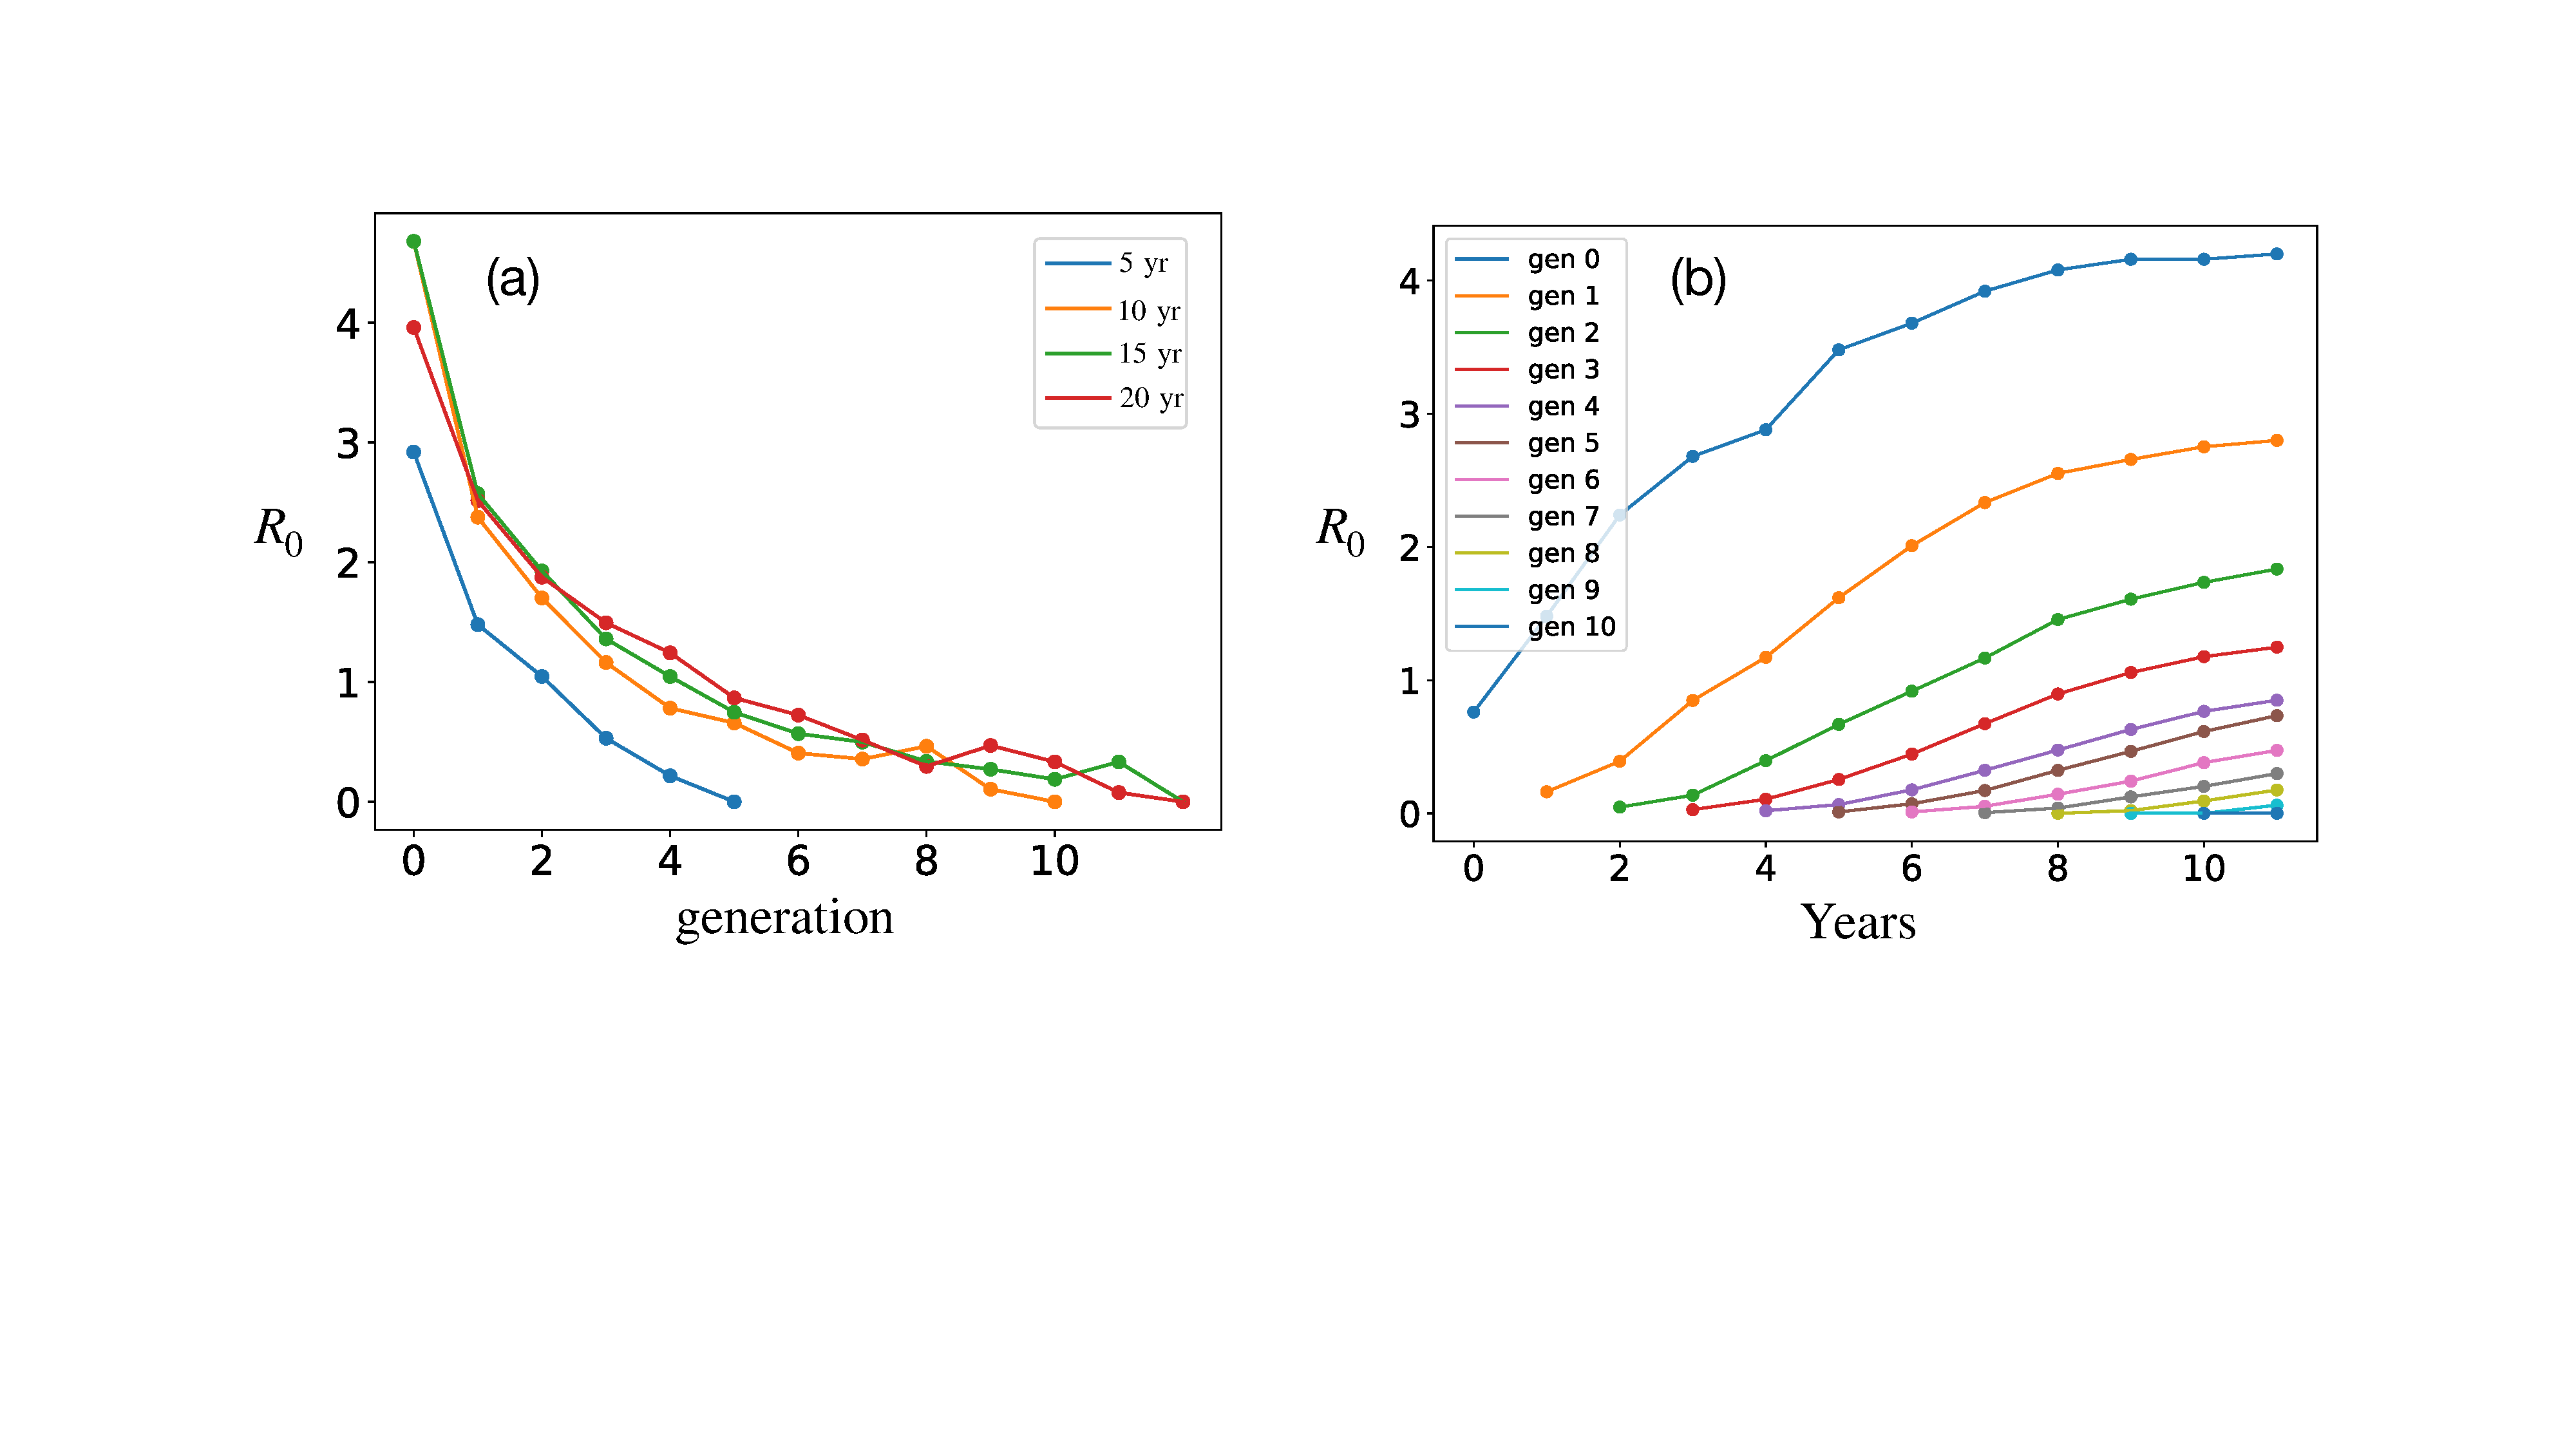
\includegraphics[scale=0.3]{chapter6/figures/fig5-R0-def.pdf}
    \caption{Contact-tracing $R_0$ in the seasonal $SEIR$ model. (a) The average number of secondary infections are shown for ash infected in the $n^{th}$ generation after outbreak (b) The average number of secondary infections is shown against the years after outbreak for different generations $0-10$.}
    \label{fig:SEIR-R0-definition}
\end{figure}

From Figure \ref{fig:SEIR-R0-definitio}(a-b) we can see the familiar saturation of $R_0$ for later generations. The decline in $R_0$ with each generation can be understood by the decline in susceptible ash with time. The first generation infected ash, at $t=0$, have a higher number of susceptible neighbours available to infect, which declines in time. The saturation point of $R_0$ mirrors the infectious lifetime which, in this model are taken to be exponentially-distributed with mean $\lambda=5\ \mathrm{yr}$. In light of better data, this choice of distribution and parameterisation could be updated. 

It makes sense to define a measure for $R_0$ based on the first generation of infections, given that the first generation has, on average, a higher $R_0$. Choosing an $R_0$ in this manner gives us an upper-bound of invasiveness, which for control, is better than an under-estimate:

\textit{The results of this, and the proceeding chapter, therefore, are based on the average number of first generation infected ash.}

Lastly, a suitable domain size $5\mathrm{km} \times 5\mathrm{km}$ was chosen to measure the $R_0$ for first generation infected ash over a $10$ year period. Primarily, this choice was taken for two reasons: 1) larger domain sizes beyond $5\mathrm{km} \times 5\mathrm{km}$ incur increasingly larger computer run times 2) there is little dependence of $R_0$ at, or beyond, this domain size or most values of $\beta$. Although, as shown in Appendix \ref{a:seir-with-L}, it is possible to under-estimated $R_0$ for high values of $\beta$, albeit slightly.

\section{Informed ash host distribution}

Up to this point, a thorough description of the host data set has been omitted. Ash densities are parameterised by modelled ash abundance data provided by \cite{hill.data}. The canopy cover datasets produced by \cite{hill.data} combine a number of different data sources that cover parts of Great Britain, regression methods are then used to extrapolate canopy cover over the whole of Great Britain\footnote{Previously in chapter chapter \ref{fig:ch4_uk_spread}, the oak canopy cover dataset given by \cite{hill.data} was used in conjunction with the SLM toy model; the insights from doing this then motivated the construction of a generic $SIR$-based dispersal model in chapter \ref{ch5:dispersal-model}.}. Conveniently for the present chapter, ash happened to be among the most accurate data sets given by \cite{hill.data}. For a more in-depth description of the methods used by \cite{hill.data} and a review of host data in general, see chapter \ref{chapter:lit-rev}.

\begin{figure}
    \centering
    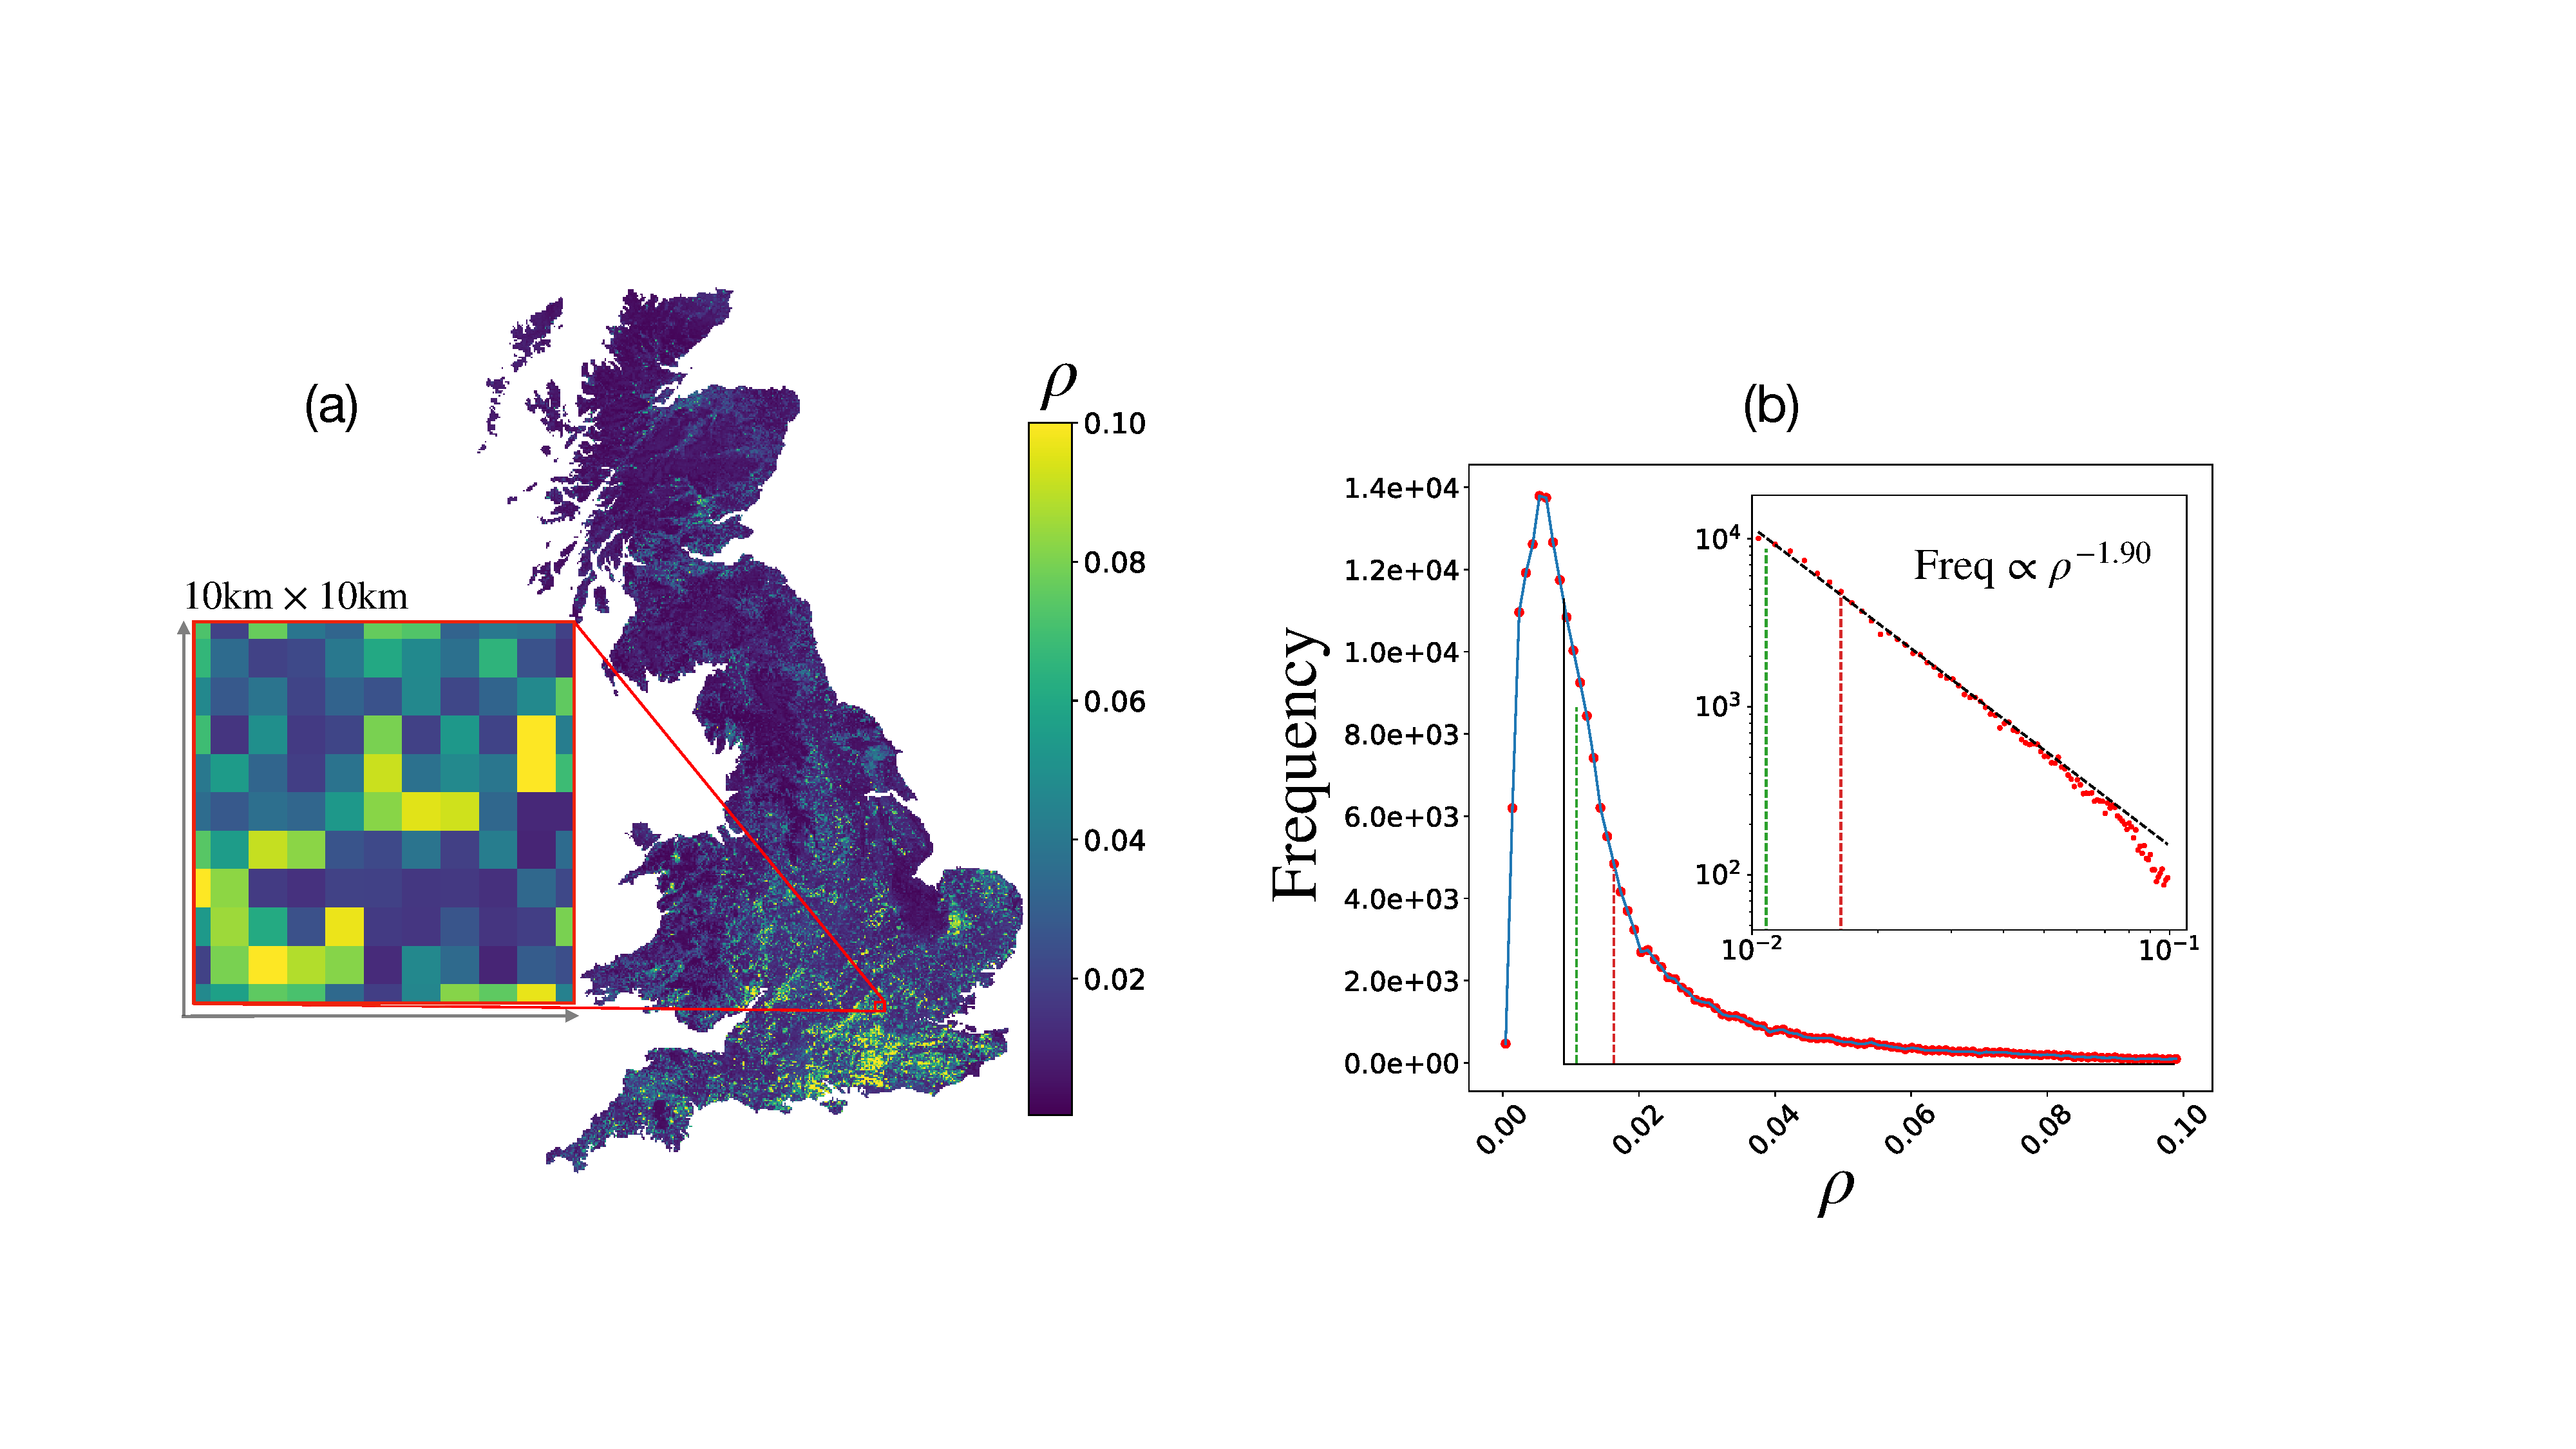
\includegraphics[scale=0.30]{chapter6/figures/fig3-ash-data.pdf}
    \caption{Ash canopy cover data, as modelled by \cite{hill.data} converted into a density. (a) a map of ash densities at a resolution of $1\mathrm{km} \times 1\mathrm{km}$ (b) the distribution of ash density over Great Britain, the inset shows a inverse power law behaviour.}
    \label{fig:ash-host-data}
\end{figure}

Figure \ref{fig:ash-host-data}(a) shows a density map of ash, at a resolution of $\mathrm{1km}\times \mathrm{1km}$, produced from abundance data given by \cite{hill.data}. From Figure \ref{fig:ash-host-data}(a), the south of England contains the highest concentration of high-density ash patches and ash become progressively less abundant in Scotland and coastal locations, in western Whales for example. A higher density of ash can be expected to yield a higher number of secondary infections, in line with the results of chapters \ref{ch3:two-param-model}-\ref{ch5:dispersal-model}.
 
The frequency distribution is shown in Figure \ref{fig:ash-host-data}(b) and reveals that the average density of ash in Great Britain is $\rho=0.017$ and that few locations support densities of $\rho=0.10$ and over\footnote{In the original $2.2\times 10^4$ $1\mathrm{km^2}$ data points, there were a handful of outlier points with densities in the interval $\rho \in [0.10, 0.30]$ which were excluded from the analysis.}. Between the limits of $\rho \in [10^{-2}, 10^{-1}]$, the frequency distribution in Figure \ref{fig:ash-host-data}(b) follows a power law of the form $\sim \rho ^{-k}$, as evident from the linearity on the logarithmic inset axes. The distribution had a fitted exponent of $k=1.90$, shown by the dashed black line. Intriguingly, this observation is suggestive of self-similarity in the data.

Two modifications had to be made to the modelled ash canopy cover data in order to complement the $SEIR$ model. Firstly, the raw abundance values were re-scaled into a dimensionless tree density $\rho$. The same process was outlined in chapter \ref{ch5:dispersal-model} i.e. by converting the units $\mathrm{ha/km^2}$ to kilometre-squared of ash cover per kilometre-squared of land. Secondly, the map resolution has to be re-scaled to reflect the intrinsic spatial scale of local wind-borne dispersal, this topic is resumed below in section \ref{ch6:re-scaling-host-data}, when ADB $R_0$-maps are constructed over Great Britain.

\section{Constructing $R_0$-maps over Great Britain}

In this section, $R_0$ values of the $SEIR$ model of ADB will be projected onto the host distribution of ash, given by \cite{hill.data}, to create $R_0$-maps. Doing so will permit the investigation of a novel control strategy. But first, to accurately project $R_0$ values onto the host distribution, the spatial and temporal scale of pathogen transmission in the $SEIR$ model must be made to match the domain resolution and the infectious lifetime of the pathogen, respectively. This requires a re-scaling of the host distribution shown in Figure \ref{fig:ash-host-data}.

\subsection{Re-scaling the host distribution}
\label{ch6:re-scaling-host-data}
% update in accordance with new figure
A choice was made to re-scale the pixel size of ash density in Figure \ref{fig:ash-host-data}(a), from $1\mathrm{km} \times 1 \mathrm{km}$, to $5\mathrm{km} \times 5 \mathrm{km}$. In the local scale field study conducted by \cite{grosdidier2018tracking}, fungal spores were detected at a maximum distance of $500\mathrm{m}$ away from a known source of infection. So on the surface, the original $1\mathrm{km} \times 1 \mathrm{km}$ resolution of the abundance data, as reported by \cite{hill.data}, appears reasonable. However, with moderate-high values of $\beta$ the power law $SEIR$ model demonstrates that singular jumps can exceed $1\mathrm{km}$ and since we cannot know $\beta$ for sure, it is desirable to air on the side of caution and re-scale the domain such that pixels represent larger spatial areas. In doing so, the resolution is lowered along with the level of spatial-structure. 

Suppose two patches of land, having tree densities above the threshold, $R_0 = 1$, are separated by an intermediary patch below the threshold. If we are not careful, dispersal could traverse the below-threshold patch within a single jump, even at local spatial scales. As such, we must choose a domain resolution that gives some assurance that, at the local scale, wind-dispersed spores cannot jump over whole patches with singular jumps. As always, there is the possibility that spores disperse more considerable distances, from mainland Europe to Great Britain, for example, \cite{freer2017tree, wylder2018evidence}. Nevertheless, this chapter aims at targeting dispersal at local scales, and LDD can be omitted for now.

Ensemble simulations can measure the maximum dispersal distance by averaging the maximum distance of secondary infections. Figure \ref{fig:max_dist_vs_R0} shows of the maximum distance traversed by the pathogen for different values of $\beta$ over a large domain, $20\mathrm{km^2}$, in a single year\textemdash or jump. The ensemble simulations shown in Figure \ref{fig:max_dist_vs_R0} start from a small number of infected trees at the centre of the domain and contrast the difference between inverse power law and Gaussian models\footnote{This is indicated by the difference in subscript on $\beta$. Technically, both are models in their own right, so a comparison between both of them with the same value of $\beta$ does not make sense. Although both models cannot be compared directly, insight can be gained by comparing model behaviours over the same $R_0$ axis.}, (a) and (b) respectively. 
\begin{figure}
    \centering
    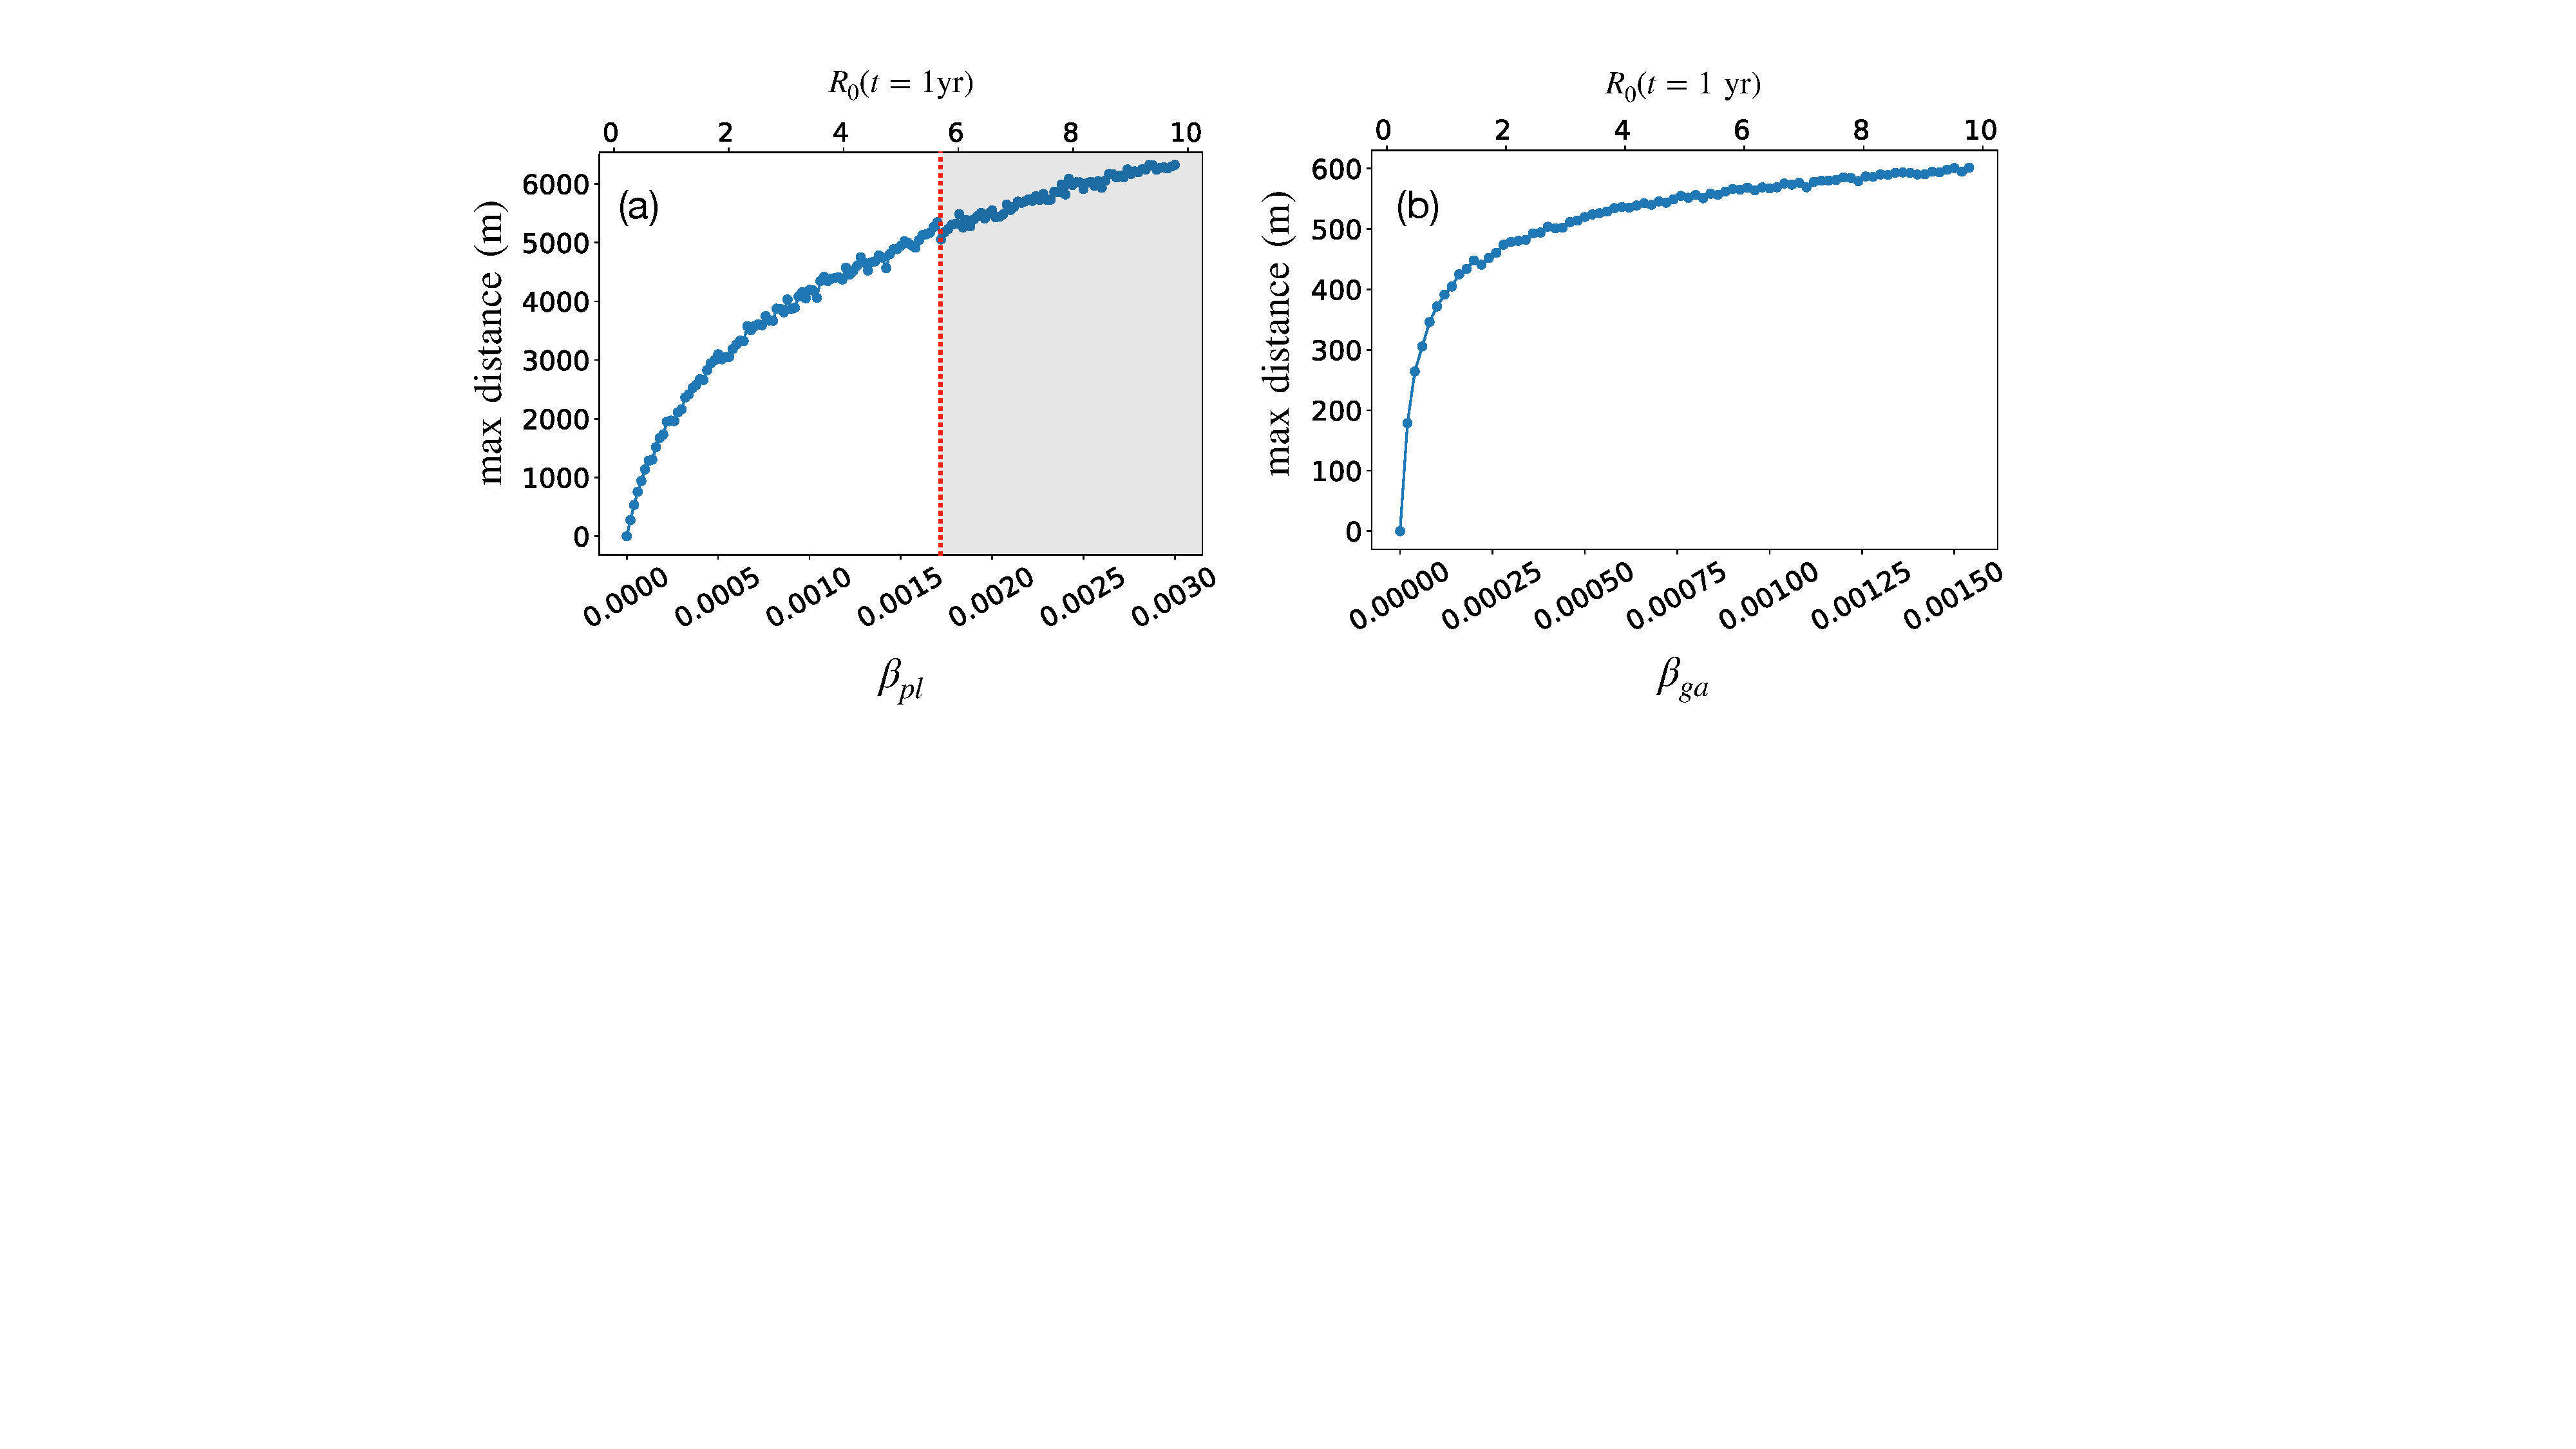
\includegraphics[scale=0.33]{chapter6/figures/fig5-beta-vs-max_d.pdf}
    \caption{The maximum distance that can be be traversed by the pathogen in a single jump is shown against different values of $\beta$. (a) the inverse power law based dispersal (b) the Gaussian dispersal.}  % update x10-4 for ga, update 
    \label{fig:max_dist_vs_R0}
\end{figure}

Interestingly, dispersal in the Gaussian model can be seen to level off between $500-600\mathrm{m}$ in line with the results from \cite{grosdidier2018tracking}, whereas, for power law dispersal, dispersal continues to rise. No doubt, this observation reflects the thin-tailed Gaussian and fat-tailed inverse power law dispersal kernels. For the exact value of $R_0$, inverse power law model can be seen to travel much further than Gaussian model and echos the difficulty of controlling fat-tailed dispersal \cite{WEBIDEMICS}, and more broadly, LDD.

For a $5\mathrm{km} \times 5 \mathrm{km}$ host distribution, we can therefore place an upper limit on $\beta$, indicated by the shaded region in Figure \ref{fig:max_dist_vs_R0} (a). If an infectivity parameter surpasses $\beta = 0.0016$, the pathogen has potential to jump over $5\mathrm{km} \times 5 \mathrm{km}$ patches and infect non-nearest neighbours. In this scenario, patches either need to be re-scaled to larger values, or the neighbourhood of interaction made non-local, as in \textcolor{red}{cite non-local R0 maps, Gilligan.} Fortunately for us however, the reproduction ratio of $R_0=6$, shown in Figure \ref{fig:max_dist_vs_R0} (a) indicates that infectivity parameters of $\beta = 0.0016$ and above are likely too high\footnote{\textcolor{red}{The value of $R_0$ shown in Figure \ref{fig:max_dist_vs_R0} (a) was measured over one sporulation season. If $R_0$ for this value of $\beta$ was measured over the mean life-time of an infected tree, we could expect to see exceedingly high, and probably unrealistic, values of $R_0$. To put this into context, the highest known case of $R_0$ is measles that...}}.

\subsection{Tree density and $R_0$}

The typical relationship between $R_0$ and tree density $\rho$ is shown in Figure \ref{fig:R0-map-generation}(a) for the inverse power law dispersal model. However, all four ADB model variants (two dispersal and two sporulation models) display the same linearity\textemdash also explored in chapter \ref{ch5:dispersal-model}. In Figure \ref{fig:R0-map-generation}(a), the regime of pathogen extinction is indicated by the horizontal red line, along with two vertical lines that correspond to a critical `density threshold' denoted by $\rho_c$ (equivalent to the threshold $R_0 = 1$). When used in conjunction with the data-set from \cite{hill.data}, Figure \ref{fig:R0-map-generation}(a) represents an appropriate projection of $R_0$ over the map of Great Britain.

\begin{figure}
    \centering
    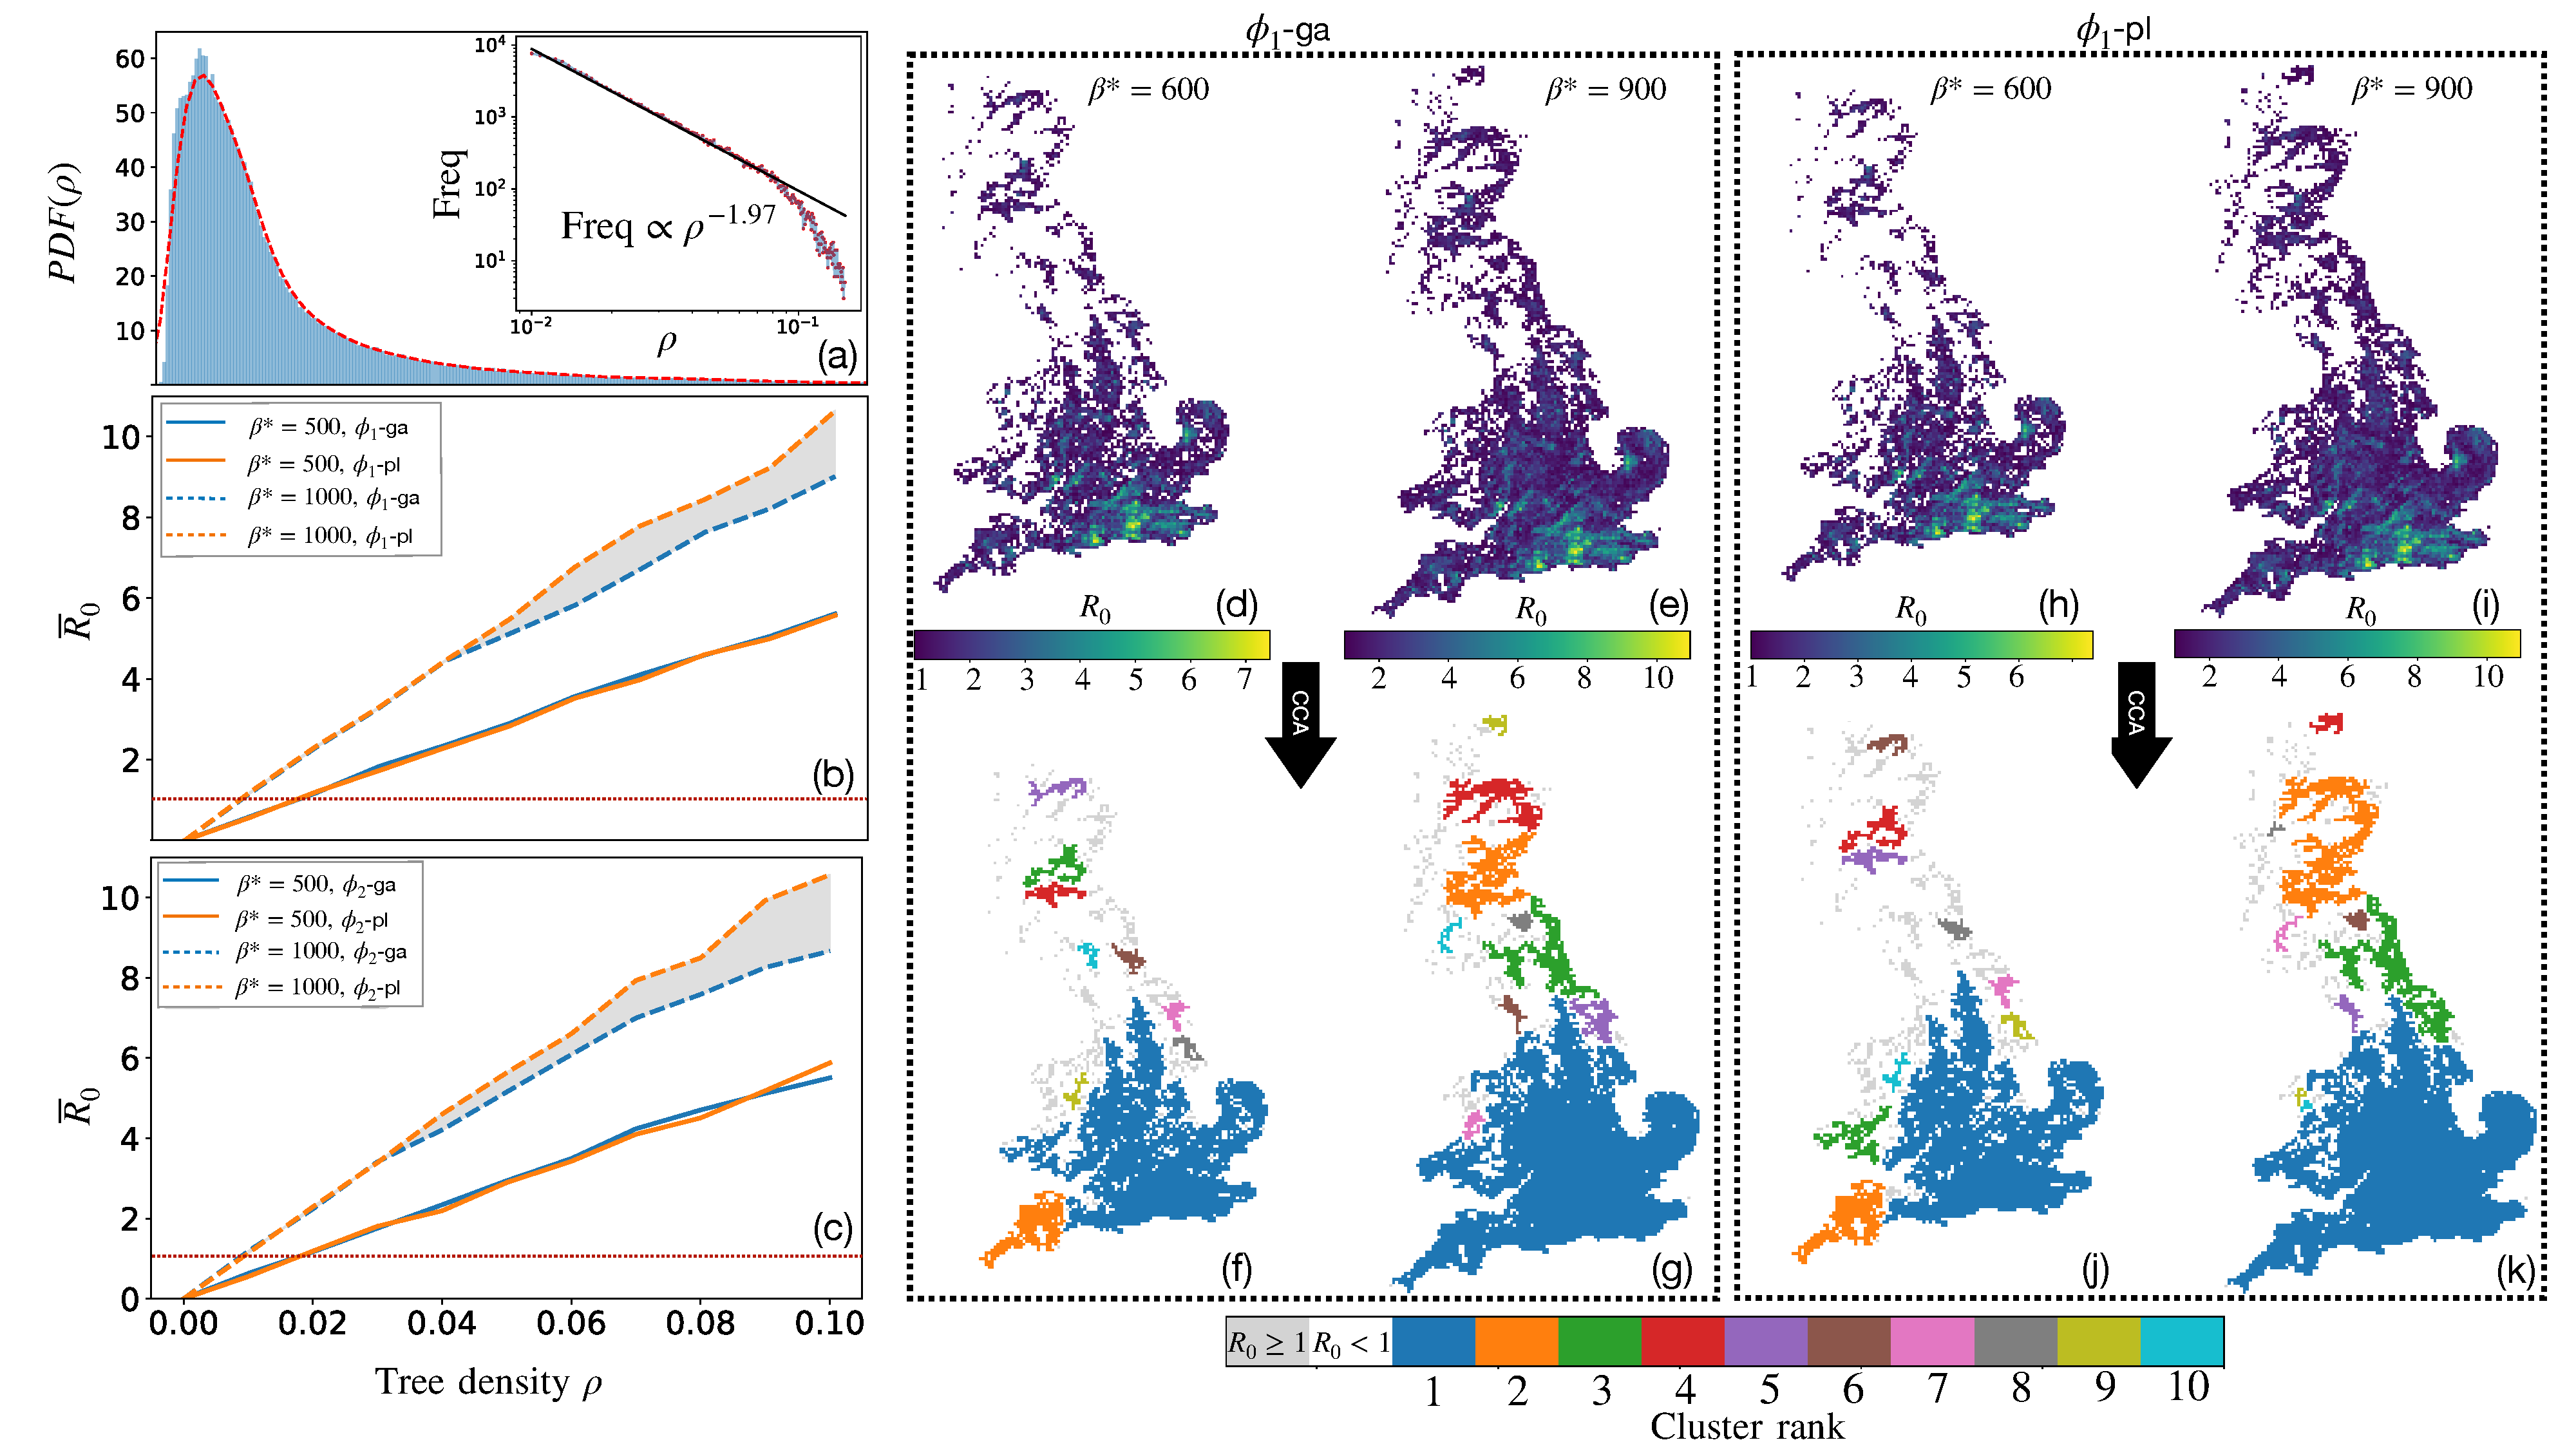
\includegraphics[scale=0.55]{chapter6/figures/fig6-R0-map-generation.pdf}
    \caption{Generating $R_0$ maps for ADB over Great Britain. (a) Ensemble-averaged results of $R_0$ are plotted against the tree densities informed by \cite{hill.data}, revealing a linear relation between $R_0$ and $\rho$. (b-c) Projecting $SEIR$ inverse power law $R_0$ values onto the re-scaled $5\mathrm{km} \times 5 \mathrm{km}$ ash host-distribution for two values of $\beta_{pl}$. Patches of land below $R_0 = 1$ are shown as white space. (d-e) The top $10$ largest connected, and susceptible, $R_0$-clusters that are present in maps (b-c).}
    \label{fig:R0-map-generation}
\end{figure}

Figures \ref{fig:R0-map-generation}(b-d) show the reproductive ratios of Figure \ref{fig:R0-map-generation}(a) projected onto the host distribution of ash. 
For all variants of the $SEIR$ model, $R_0$-maps look similar, albeit with different $\beta$ values, see Appendix \ref{fig:a-R0-maps-SEIR-variants}. 
The values of $\beta$ shown in Figures \ref{fig:R0-map-generation}(b-d) correspond to the values of $\beta$ shown by blue and orange lines in Figure \ref{fig:R0-map-generation}(a) respectively. 
Under the influence of a more infectious pathogen, larger areas of the ash population become susceptible by supporting the growth and reproduction of the pathogen, illustrated by the difference in patch density in Figures \ref{fig:R0-map-generation}(b-c). 
All locations below the transmission threshold $R_0=1$ were given numerical values of zero and are depicted by inland white space.

Suppose that the two lines in Figure \ref{fig:R0-map-generation}(a) represent an upper and lower bound of invasiveness in $\beta$. 
In this scenario, epidemic uncertainty is captured in the divergence between lines, depicted by the shaded grey area and vertical arrow. 
By projecting $R_0$ onto the host distribution informed by \cite{hill.data}, epidemiological uncertainty can be conveniently visualised by contrasting clear differences between $R_0$-maps in Figures \ref{fig:R0-map-generation}(b-c). 
The next section presents a means to identify clustering in $R_0$-maps.

\subsection{Clustering in the $R_0$ map}

From Figures \ref{fig:R0-map-generation}(b-d), landscape-level heterogeneity and high-risk areas can be loosely identified.
However, visualising which pixels connect to form large clusters is non-trivial. 
An image processing technique, called connected component analysis (CCA) \cite{CCA1, CCA2}, was used to identify and label susceptible clusters and simplify the $R_0$-map. 
The Python-SciPy package `ndimage' \cite{scipy} was used to implement CCA via the function `label'. 
Doing so labelled all susceptible neighbours as connected members of the same cluster, according to a structuring element \cite{liang1989erosion}. 
That is, if two susceptible patches of ash lie within the same neighbourhood, defined by the structuring element, they are connected members of the same cluster\footnote{Structuring elements have their roots in shape and image analysis \cite{23111}, where they define how distinct binary shapes connect to form images \cite{liang1989erosion, nachtegael2001connections}}. 
More information on structuring elements and CCA can be found in Appendix \ref{a:R0-map-construction}.% To fill in Appendix

Moore and Von-Neumann neighbourhoods were chosen as structuring elements to classify connected components\textemdash a comparative look exploring the differences between Von-Neumann and Moore 
structuring elements is resumed below in section \ref{R0-over-beta}.  
Figures \ref{fig:R0-map-generation}(d-e) show the top 10 largest connected $R_0$-clusters, by area, that are present in the $R_0$-maps of Figures \ref{fig:R0-map-generation}(b-d) for two different values of $\beta$ 
according to the Moore neighbourhood.
Increasing the infectivity parameter $\beta$ leads to a more connected map, as demonstrated by the larger dominating cluster in Figure \ref{fig:R0-map-generation}(e).

\subsection{Interpreting susceptible $R_0$-clusters}
Given that disease gradients can extend over $10-1000\mathrm{km}$, we cannot preclude the possibility of secondary infections spreading between clusters.
Alongside jumping directly over below-threshold patches, the pathogen may also use intermediary trees inside below-threshold patches as stepping stones and jump between clusters indirectly. 
Conceptually, this has been described for pathogens jumping between crop fields \cite{Gilligan-disease-management} and more abstract modelling work \cite{wingen2013long}.
In a simplified interpretation, the model presents two distinct types of spread, within-cluster and between-cluster spread. 

Patches below the threshold present a natural barrier to ADB spore dispersal between clusters, for two reasons: 
1) Below-threshold patches do not support high levels of infected biomass, spore dispersal emanating from these patches will therefore be lessened.
2) The domain resolution, configured in section \ref{ch6:re-scaling-host-data}, ensures that no secondary infections will result for the parameter values and spatial scale under consideration in the seasonal $SEIR$ model of ADB.
Likewise, susceptible and connected $R_0$-clusters reveal which regions in Great Britain are likely to be the most severely devastated, and
where transmission between neighbouring patches is tightly coupled.

Here, within-cluster connectivity is sufficient for uninhibited spore-dispersal between nearest-neighbour patches in the $SEIR$ model of ADB, 
and where disease may spread over large spatial scales even without the need for LDD\textemdash without directly, or indirectly, jump between nearest-neighbours.
Thus, clustering in the $R_0$-map allows high-risk areas to be conveniently identified in a simplistic manner. 
The connectivity between clusters is the subject of chapter \ref{ch7:pde}, for now, we consider only within-cluster connectivity.

% Do I include these paragraphs ? - perhaps the chapter summary / discussion may be sufficient
% In this model, the epidemic spread within an $R_0$-cluster of ash can be reduced to a `\textit{percolation-like}' problem, with the caveat of heterogeneity. If susceptible patches of ash were homogeneously distributed, a minimum number of susceptible (or `open' in percolation theory) positions would define a critical density, and a spanning cluster would percolate through the domain, as laid out in chapter \ref{ch3:two-param-model}. A similar picture is painted within the $R_0$-maps shown in Figures \ref{fig:R0-map-generation}(d-e). Figure \ref{fig:R0-map-generation}(d) depicts a fragmented domain at $\beta_{pl}=...$, increasing the pathogen infectivity to $\beta_{pl}=...$ yields a much larger '\textit{dominating}' $R_0$-cluster, as shown in Figure \ref{fig:R0-map-generation}(e).

% Classical percolation theory requires lattice points to be independently open or closed, with no dependence on the state of nearest neighbours. So, strictly speaking, the analogy to percolation breaks down because the susceptibility of a given patch of ash is likely dependent on its neighbours $R_0$-value; as can be seen in Figures \ref{fig:uk-mapping}(d-e), particularly in the south of England where ash densities are high. 
% Heterogeneity in the $R_0$-map becomes particularly useful in the the next chapter, where we investigate a potential strategy of landscape-level control based on disrupting epidemic connectivity and fragmentation.
% Before we can move towards epidemic control, it is desirable to understand $R_0$-clustering more fully.

\subsection{$R_0$ Cluster-distributions}
\label{R0-over-beta}

For each value of $\beta$, an $R_0$-map will have a distribution of different clusters; 
this is true except for two edge cases: $\beta$ is too small or too large, in which case there will be no (or trivially small) clusters or one singular cluster that covers the domain.
A rank-ordered list of cluster-sizes is shown in Figure \ref{fig6:cluster-size-distributions} for all $SEIR$ ADB model variants.

All model variants display the same essential behaviour. 
For lower values of $\beta$, more distinct clusters are present and lower-ranked clusters are on average larger than higher values of $\beta$,
as demonstrated by comparing size-difference between the red and blue colored distribution.
As $\beta$ is increased, the domain becomes more connected, resulting in one large, dominating $R_0$ cluster that covers the domain alongside a handful of small pockets.

\begin{figure}
    \centering
    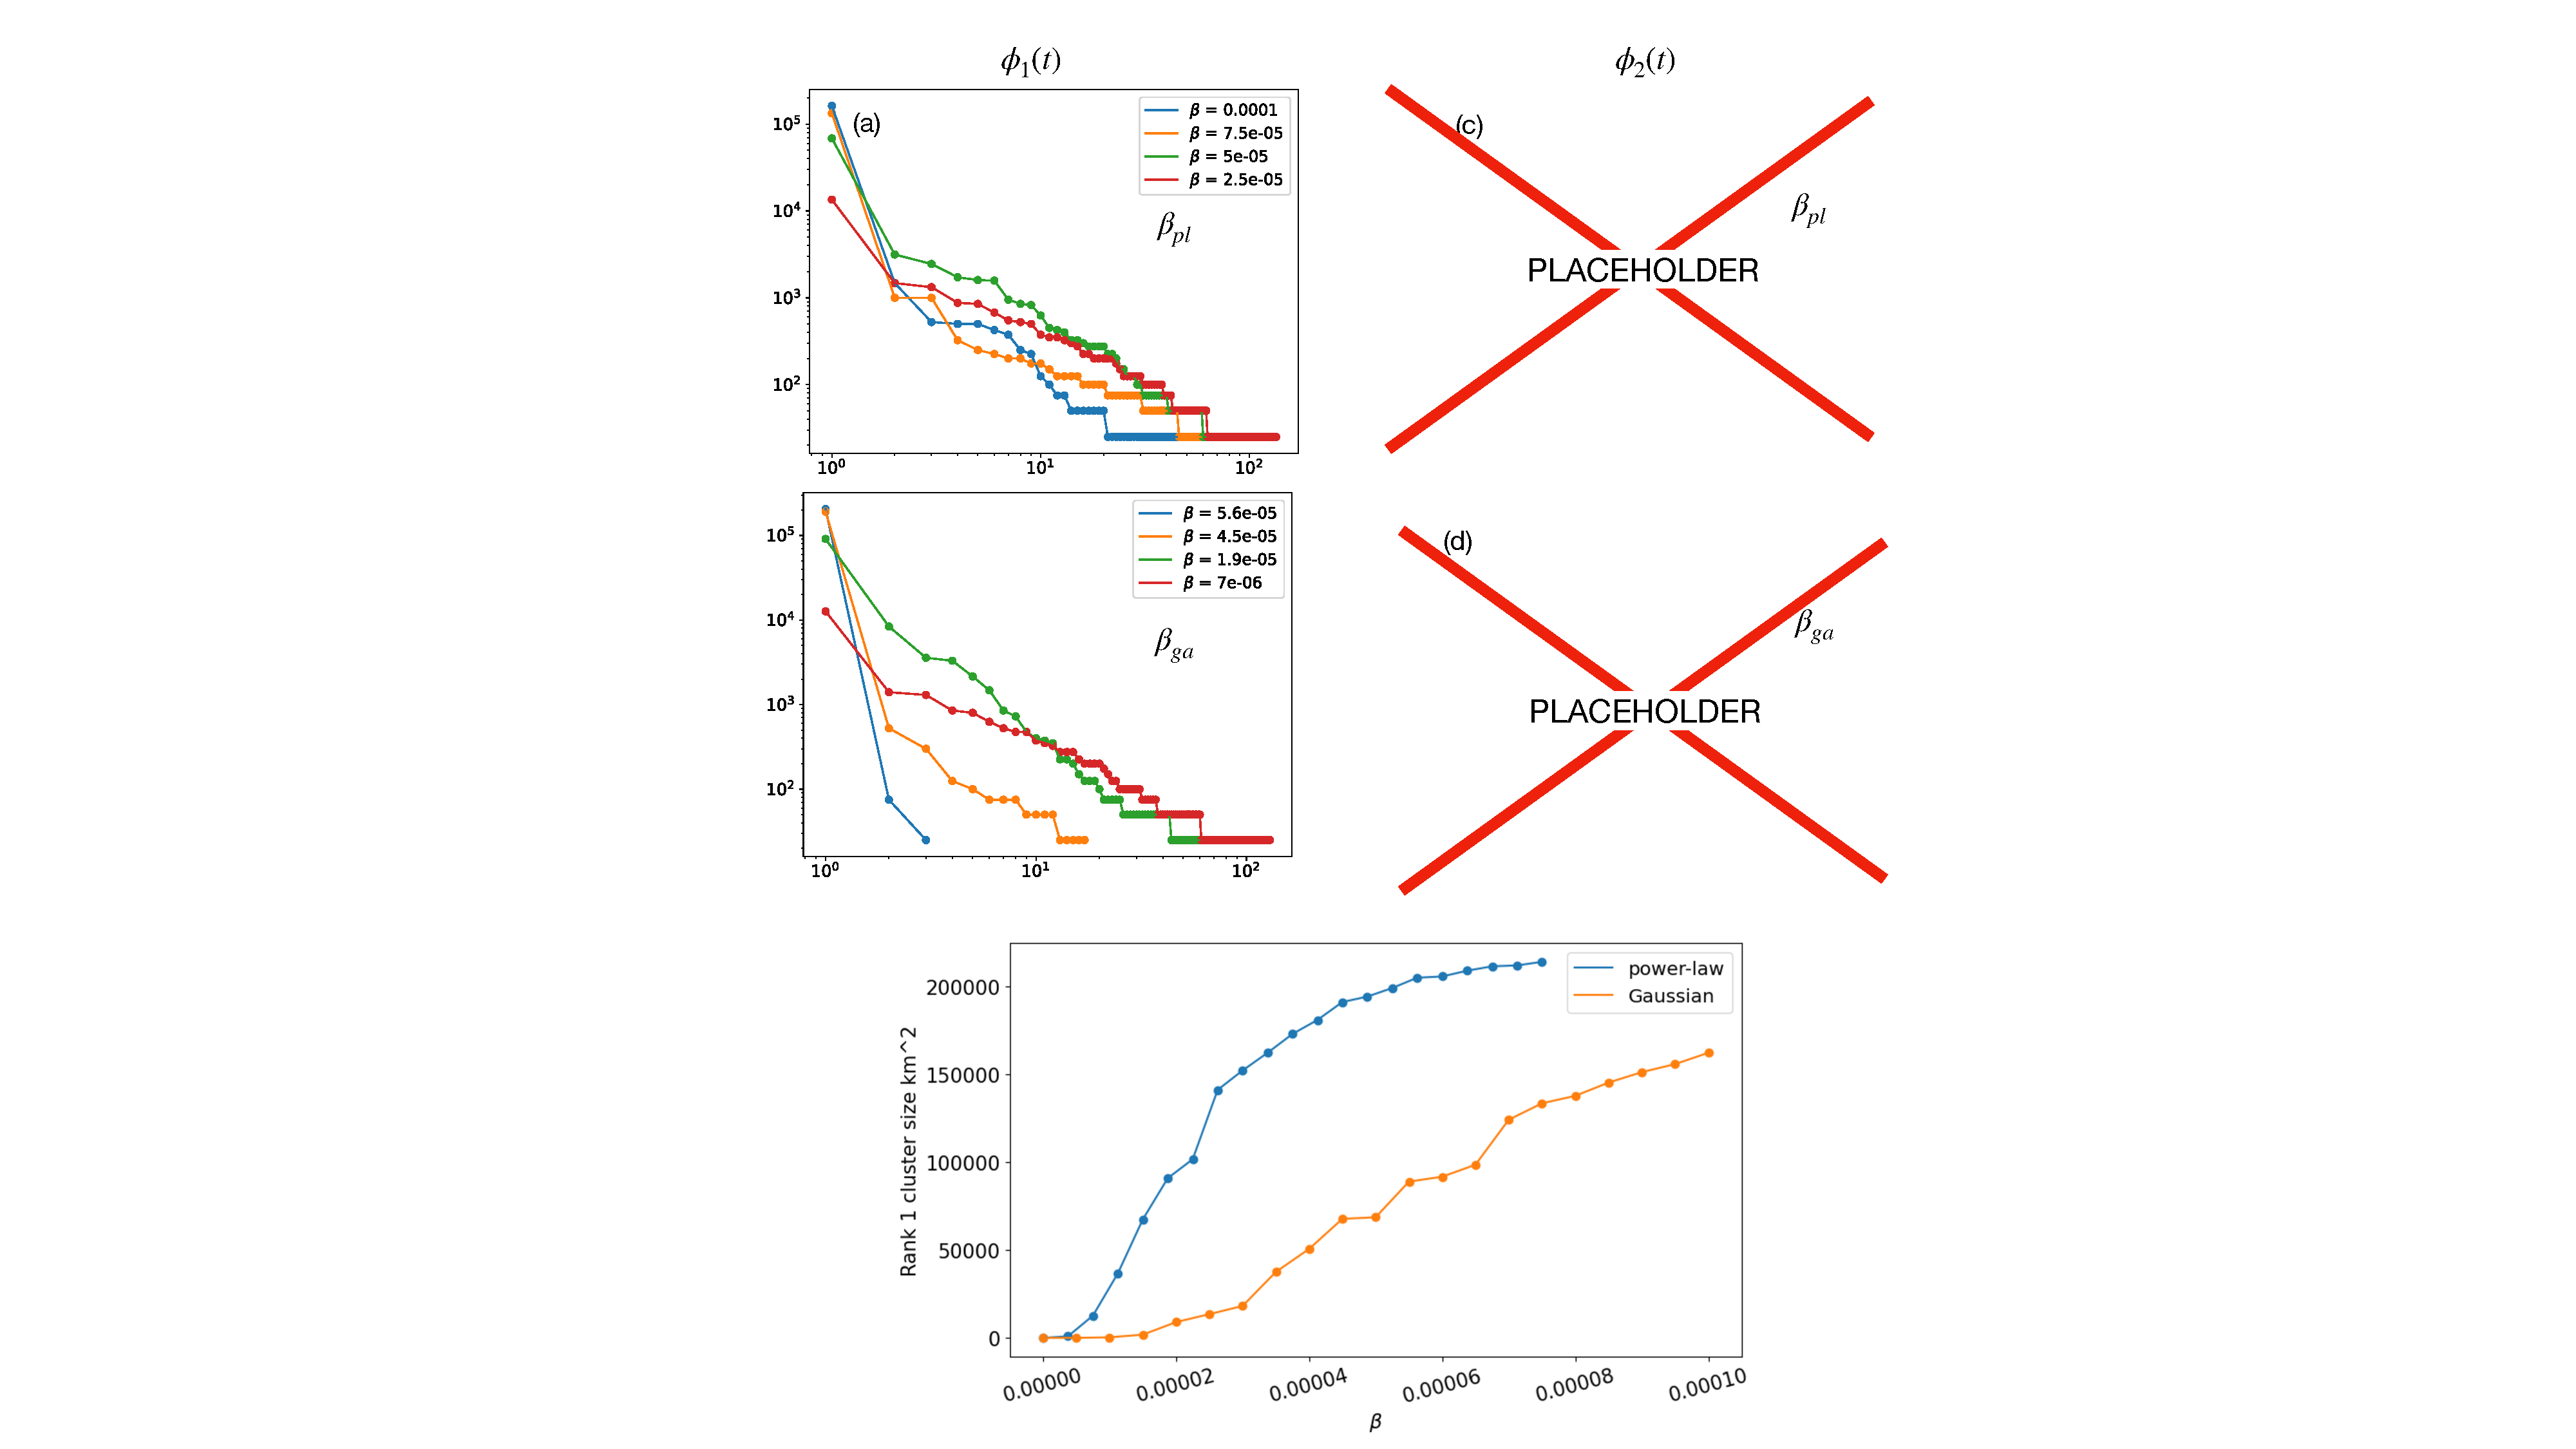
\includegraphics[scale=0.50]{chapter6/figures/fig6-cluster-size-distribution.pdf}.
    \caption{Cluster size-distributions for the inverse power law (a-b) and Gaussian (c-d) dispersal and sporulation models. A rank-ordered list of connected-cluster size is shown against different values of infectivity $\beta$. As $\beta$ grows larger, the number of clusters decrease until one large dominating cluster covers Great Britain.}
    \label{fig6:cluster-size-distributions}
\end{figure}

Interestingly, the disparity between clusters-size, and the distance between clusters could be used to give insight into
which spatial scale is the dominant driver of disease spread.
The more sparsely distributed\textemdash and thus fragmented\textemdash the $R_0$-map, the more important LDD becomes as the driver of between-cluster spread.
Crucially, accessing the relative importance of spatial scale between disease drivers would rely on a fitted value of $\beta$,
and the knowledge that ADB is estimated to spread with impunity and kill over $85\%$ of ash in Great Britain.

\begin{figure}
    \centering
    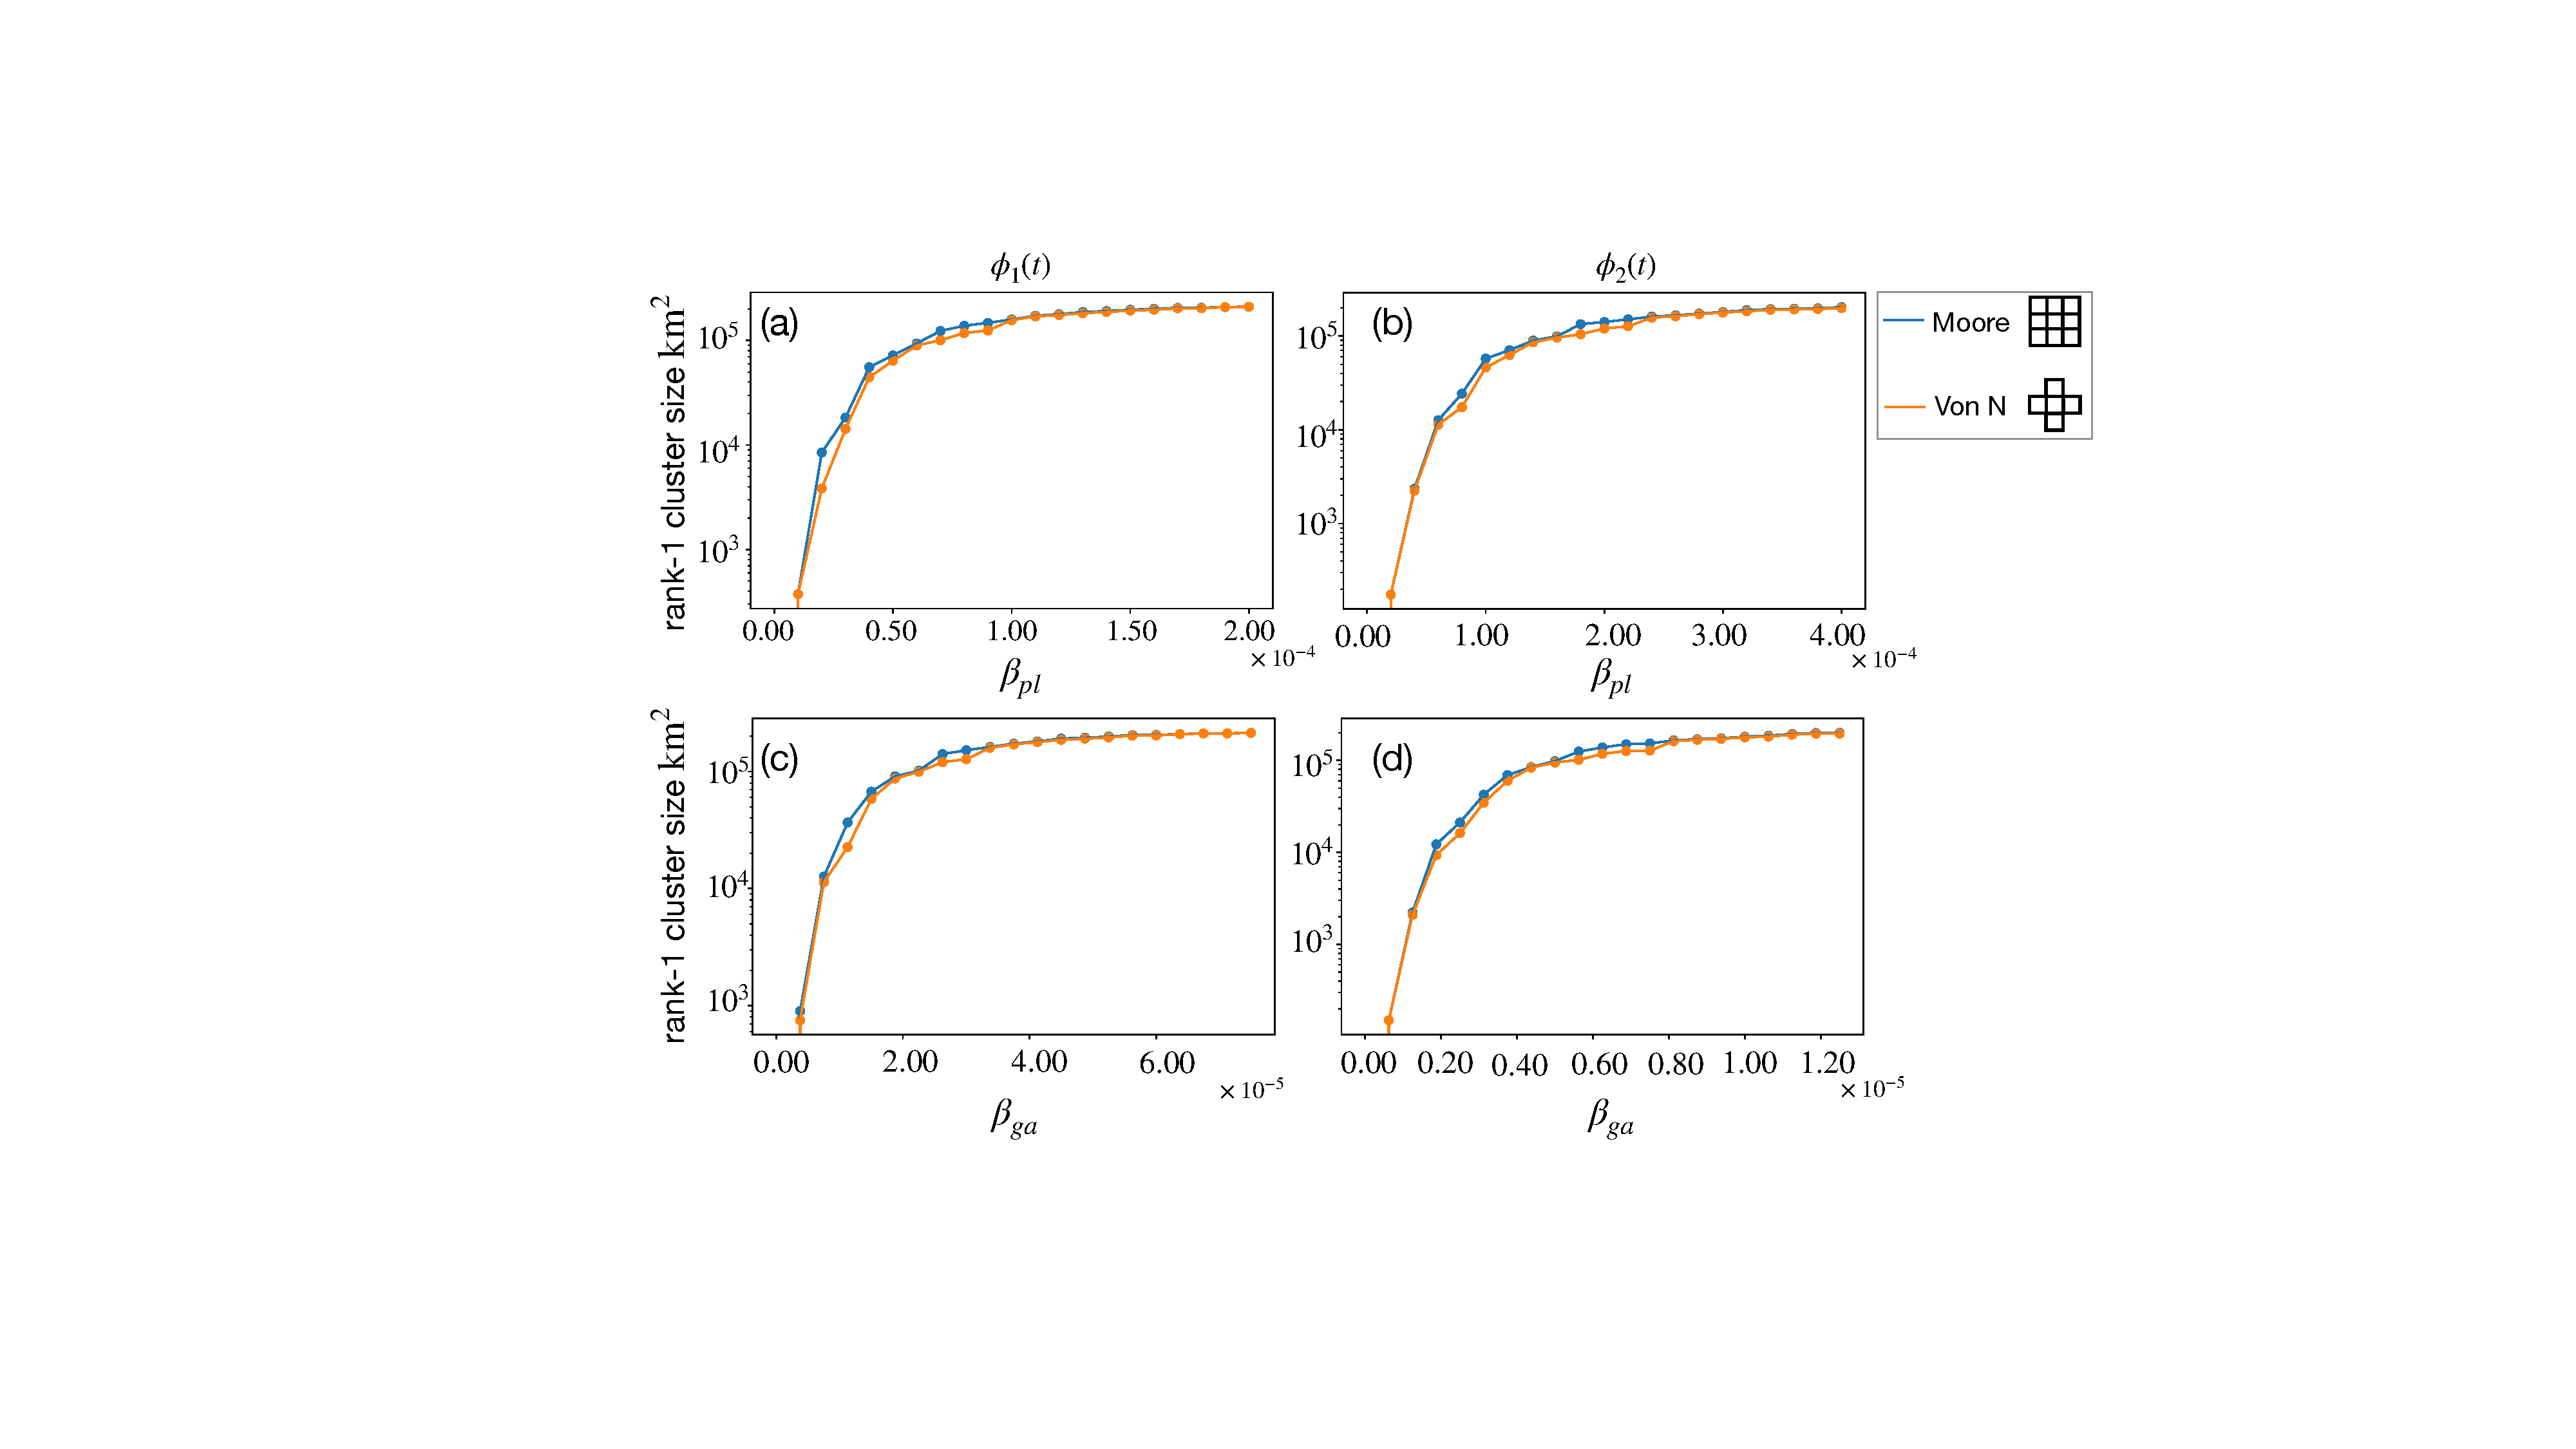
\includegraphics[scale=0.45]{chapter6/figures/fig6-largest-cluster-over-beta.pdf}.
    \caption{The largest connected cluster present in the domain shown over infectivity $\beta$ and two structuring elements, von Nuemann and Moore. (a-b) The inverse power law dispersal model for sporulation functions $\phi_1$ and $\phi_2$ (c-d) The Gaussian dispersal model for sporulation functions $\phi_1$ and $\phi_2$. The von Nuemann structuring element leads to slightly smaller cluster sizes.}
    \label{fig6:largest-cluster-over-beta}
\end{figure}

Figure \ref{fig6:largest-cluster-over-beta} shows how the largest susceptible cluster in Great Britain depends on $\beta$ and the choice of structuring element. 
As $\beta$ increases, the largest $R_0$-cluster size increases. 
For sufficiently large $\beta$, a large single cluster
\footnote{To put the scale of Figure \ref{fig6:largest-cluster-over-beta} into perspective, the approximate area of Great Britain is $\approx 2.2 \times 10^5$.} 
spans Great Britain. 
In Figure \ref{fig6:largest-cluster-over-beta}, cluster-size scarcely depends on either von Neumann or Moore structuring elements. 
Although, a von Neumann gives rise to slightly smaller clusters\textemdash on account of four missing corner connections. 

For all ADB model variants, a sharp rise in cluster-size can be seen to occurs over a over a narrow range of $\beta$ values.
Figure \ref{fig6:largest-cluster-over-beta} therefore demonstrates how sensitive the model can be to changes in $\beta$, and that map-connectivity deponents strongly on the invasiveness of the pathogen.
From these observations, the importance of epidemiological uncertainty in the model becomes clear.
For certain regimes of $\beta$, a small deviation in can produce a large rise in cluster-size, extending over nearly an order of magnitude.

\section{Chapter summary}

% Where we consider spatial structure and others have not
% - In this chapter, we focused on disrupting local-level dispersal by implementing control at landscape-level.
% -  In this chapter we undertook the ambitious task of scaling up a small-scale model, to large spatial distances covering GB, and developed a new approach to controlling the spread of disease.
% - introduce the regime of pathogen spread we are interested in, we are not modelling continental long-range spread via upper atmosphere, nor are we interested in long-range human trade networks. We are interested in dispersal at the local level whereby passive means of wind, soil and or insects/animals. 

% link to 13 challenges: -- it is your friend...
% 1 - host data is hard to integrate into models \cite(13 challenges), we demonstrate how how this can be achieved
% 2. primed a model of multi scale, although we have not included LDD spore transport, the framework serves to include this via a more complete treatment of the structuring element
% 3. capturing time-varying infectivity is hard \cite{13 challenges},
% 4. constructing a spatial model of disease severity could help to deploy resources to known locations e.g. monitoring
%5. web api to help policy makers

These results are focused toward help policy makers implement informed decisions, about \textit{where} to control the spread of disease, based on spatial arguments, when budgets are low\textemdash as noted by \cite{time-varying-infectivity}. Our approach of spatially scaling small-scale epidemiological principles was conducted through computational, opposed to analytical, means. 

% The scaling up of our model
The scaling up of our model resembles a metapopulation model, now commonplace when modelling plant-based epidemics, but crucially our large-scale model is not dynamic. A dynamic large-scale model is indeed useful for the prediction of time-scales and the movement of disease-fronts movement; however, we suggest they might be at best less useful for optimised large-scale control, and at worse, nicely complemented by the approach we develop.

If early data through a particular region, with known data, was collected, it would be a relatively short step to fit the dispersal model and scale up the model over large distances given the seemingly simple relation to host density $\rho$.
% At the small scale we have a uniform population. However for larger scales we have considerable spatial heterogeneity.
% spatial-scale and control, over a multi-seasonal pathosystem, have been investigated for sugar beet in the UK, see \cite{doi:10.1146/annurev.phyto.45.062806.094357} for a review.

% On the SEIR model

The cyclic nature of the $SEIR$-type model constructed in this article can also find resemblance in the, well established body of literature, of crop-based epidemics. It is common-place for a field of crops to become infested, then at the end of the growing season be totally eradicated by virtue of harvesting 
% there is a surprising lack of, simplified, ash dieback models in the literature...\ciations... <-- double, triple and quadruple check!
% without host demography 
% landscape level control strategy

% multi-scale approaches have been outlined \cite{hart2020theoretical}
% multi-seasonal frameworks comprise a common theme in the spread of crop-based epidemics see  x, y, and typically involve soil-borne nematodes-based outbreaks \cite{tankam2020modelling} <- see references inside.

% \cite{time-varying-infectivity} has 
% we contend the SnIEmR model, considered over one sporulation peak, is a simplistic implementation of the SEIR-based model needed to compute an invasion threshold that represent the infection dynamics ash dieback. 
% The SEIR-based model is made more flexible, and can be readily extended or adapted to incorporate more biological realism, by virtue of splitting the E and I into multiple compartments\textemdash this is frequently done in human and animal-based models \citations..

% - time varying infectivity parameter for ADB \beta could be subject to increase in response to the warmer conditions presented by climate change \cite{magarey2005simple}
% - Interestingly, ash dieback could be adversely effected be climate change \cite{goberville2016climate}


%- Although the main result of our work was conduced over one sporulation peak, or life-cycle of ash dieback, splitting the model into various compartments was a useful and necessary step towards developing accurate large-tree species. reference  \cite{https://doi.org/10.1111/ppa.12894} alludes to multiple exposed periods being useful

%- A quantity of interest that appears frequently in the literature is the initial growth rate $r$, that is the density-independent growth at the start of any epidemic.
% See \cite{ferrandino2012time} for a review on the time-scales and sporulation of plant-based diseases.

% Fitting data to the early phases of an epidemic has been shown to give large differences in the final-size epidemic, or severity \cite{time-varying-infectivity}. However, we are only interested in a pathogens ability to invade and this can be closely approximated by measuring R0 over the fist observation (\see appendix)
% fitting....- Although, various data regarding ash mortality after years of infection have been published in various countries, as reviewed in chapter \ref{ch2:ash-dieback}.
% The variability between the particular life-cycle history followed by hosts is thought to be an important factor to consider\cite{ferrandino2012time}, and we intentionally neglected this for the purpose of simplicity...

% \footnote{A review on the landscape epidemiology of ADB \cite{doi:10.1111/1365-2745.13383} concluded that the effect of host abundance in the neighborhood of ADB decayed with distance, according to an exponential distribution with scale parameter $200\mathrm{m}$. That is, the severity of ADB symptoms depended on the surrounding abundance of ash.} 
% 

% subdividing compartments in this manner could also provide an easier implementation to hosts which become more infectious, through a greater production of spores, as the infectious cycle continues not to mention particular periods of environmental unsuitability.
%

% Accurately modelling time-varying infectivity is difficult \cite{13-challenges}, and as such, we opted for parsimony.

% Main assumptions in the method: 
% 1) Assumptions about dispersal
Dispersal over small spatial-scale is thought to predominately occur passively through wind, however other means of dispersal exist such as soil and or insects. There are many pathways a pathogen can use to spread through a landscape, including long-range dispersal, mediated through either human-trade networks %
\cite{hulme2009trade, banks2015role, chapman2017global} or dispersal in the upper atmosphere \cite{westbrook1999atmospheric, isard2005principles}.  

% \textcolor{red}{The last insightful observation from Figure \ref{fig:max_dist_vs_R0} relates to the averaging spreading velocity of ADB...}
% We assumed some regions can sustain an epidemic and some cannot, we assume that $R_0>1$ is the threshold separating these regimes.

% 2) Assumptions about R0
To our knowledge, $R_0$ has not been estimated for Ash dieback, or indeed for any large deciduous tree species, unlike for some crop-based pathogens \cite{segarra2001epidemic}. The lack of $R_0$-estimates made it hard to scrutinize which $\beta$-valued $R_0$-map would be likely to reflect reality. This gap in the body of literature is hardly surprising given the complexity of measuring time-varying infectivity rates \cite{13-challenges}. Thus, as it stands, our results hint-towards the utility of landscape-level control but come short of definitive proof.

% Looking at \cite{R0-perc-ref}, it makes me think our notion of $R_0$ is pretty simplistic. We only measure the local-level $R_0$. We do not consider $R_0$ from patch to patch. What scale we measure $R_0$ has a huge impact on what the result is. Could we rank land-patches not only on there local $R_0$ level, but also on the impact they have on there immediate neighbours ? This would, in theory be an improvement to the clustering algorithm.

% A map of $R_0$ values is useful to policy makers and plant modelers alike.

% Improvements to the model:
% 1) The algorithm
% The algorithm to target not only the critically connecting patches, but also find fragmenting lines which minimise risk at the landscape-level ? Incorporating the local impact a particular patch may have on its neighbours.
% 2) Multi-year R0 analysis
% However, we .... xyz cover all basis of using a one-season approximation. <- this leads to a risk-based argument in which we could capture a 2nd-order R0 which does, xyz. We mainly interested in a pathogens ability to invade. 

% Analysis was aired towards simplicity, a more expansive study with e.g. more sophisticated sporulation functions could be the subject of future work.

% The most important message of our work was...
% The spatial and temporal scale of the control-strategy should match intrinsic spatial and temporal scale of the invasion. <- Hence R0 measured over one season. 

\textbf{Assumptions}
\begin{itemize}
    \item Infectious, dead leaf litter was assumed to fall close to infected ash, and ash were taken as the site of fungal dispersal. In reality dead leaves could themselves disperse. 
    However, the dispersal parameterisation from \cite{grosdidier2018tracking}
    Omitting leaf dispersal simplified the model and given informed parameterisation by from \cite{grosdidier2018tracking} bared no influence the scale of dispersal
    \item leaf dispersal has been studied by \cite{https://doi.org/10.1890/0012-9658(2006)87[2306:MLDIMH]2.0.CO;2, staelens2003model}
    \item no host demography link to $R_0$
    \item The transition probability $\beta$ is constant throughout the life-time of infected ash. 
\end{itemize}

% our modelling approach and results are in their infancy,  

% Last remarks and future modelling work:
To our knowledge, there is a surprising lack of spatio-temporal ADB models exist in the literature, probably because of the significant challenges involved in containment. Although our findings are far from complete, it suggests the spread of ash dieback, between spatial locations, could be reduced by preferentially targeting sites to minimise epidemiological connectivity. Not surprisingly, more work will need to be done to ascertain the degree to which this strategy could impede the spread. 



